% Clase del documento
\documentclass[12pt,twoside,titlepage]{report}





%%%%%%%%%%%%%%%%%%%%%%% Paquetes %%%%%%%%%%%%%%%%%%%%%%%

\usepackage[a4paper,bindingoffset=3mm,bottom=35mm]{geometry}


% Usad \usepackage[dvips]{graphicx} o \usepackage[pdftex]{graphicx} (no ambos)
%\usepackage[dvips]{graphicx} %%% para LaTeX. Las figuras deben estar en formato eps

\usepackage[colorlinks=true,pdftex]{hyperref}   %%% Opcional. Para incluir marcadores y enlaces en el pdf
\usepackage[pdftex]{graphicx}  %%% para pdflatex. Las figuras pueden estar en pdf, jpg, svg y otros formatos


\usepackage[spanish]{babel}

%\usepackage[latin1]{inputenc} % Usad en WinEdt/MikTex
\usepackage[utf8]{inputenc} % Usad en overleaf

%\usepackage[T1]{fontenc}


% Algunos paquetes útiles

\usepackage{amsmath,amssymb}
\usepackage{hyperref}
\usepackage{xcolor}
\usepackage{afterpage}
\usepackage{paralist}
\usepackage{array}
\usepackage{enumerate}
\usepackage{paralist}
\usepackage{enumitem}
\usepackage{float}
\usepackage{setspace}
\usepackage{listings}
\usepackage{algorithm}
\usepackage{algorithmic}
\usepackage{fancyhdr}
\usepackage{rotating}
\usepackage{multirow}


% Otros paquetes

\usepackage{quotchap}
\usepackage{lipsum}

%%%%%%%%%%%%%%%%%%%%%%%%%%%%%%%%%%%%%%%%%%%%%%%%%%%%%%%%






%%%%%%%%%%%%%%%%%%%%%%% Definiciones básicas %%%%%%%%%%%%%%%%%%%%%%%

\newcommand{\nombreautor}{Ángel Baeza Sánchez}
\newcommand{\nombrecoautor}{Marta Vidal González}
\newcommand{\nombrecoautorespacio}{Marta Vidal González }
\newcommand{\nombreproductor}{Eva María Pérez Lajarín}
\newcommand{\nombretutor}{María Zapata Cáceres }
\newcommand{\titulotrabajo}{Programación de un Videojuego para el Desarrollo del Pensamiento Computacional}
\newcommand{\escuela}{Escuela Técnica Superior\\de Ingeniería Informática}
\newcommand{\escuelalargo}{Escuela Técnica Superior de Ingeniería Informática}
\newcommand{\universidad}{Universidad Rey Juan Carlos}
\newcommand{\fecha}{Fecha}
\newcommand{\grado}{Grado en Diseño y Desarrollo de Videojuegos}
\newcommand{\curso}{Curso 2023-2024}
\newcommand{\logoUniversidad}{logoURJC.pdf} % logoURJC.eps

%%%%%%%%%%%%%%%%%%%%%%%%%%%%%%%%%%%%%%%%%%%%%%%%%%%%%%%%%%%%%%%%%%%%






%%%%%%%%%%%%%%%%%%%%%%%%% Otras definiciones %%%%%%%%%%%%%%%%%%%%%%%%%%

% Definiciones de colores (para hidelinks)
\definecolor{BlueLink}{rgb}{0.165,0.322,0.745}
\definecolor{PinkLink}{rgb}{0.8,0.22,0.5}
\definecolor{gray}{rgb}{0.6,0.6,0.6}


% Enlaces
\hypersetup{hidelinks,pageanchor=true,colorlinks,citecolor=PinkLink,urlcolor=black,linkcolor=BlueLink}


\newcommand\blankpage{%
    \newpage
    \null
    \thispagestyle{empty}%
    %\addtocounter{page}{-1}%
    \newpage}


% Texto referencias
\addto{\captionsspanish}{\renewcommand{\bibname}{Bibliografía}}

% Texto Índice de tablas
\addto\captionsspanish{
\def\tablename{Tabla}
\def\listtablename{\'{I}ndice de tablas}
}


\floatname{algorithm}{Algoritmo}

\newfloat{algorithm}{t}{lop}

%% Etiquetas de comentarios (tutor/alumno)
\newif\ifdraft
\drafttrue
\usepackage{subcaption}
\newcommand{\nb}[2]{
	{
		{\color{black}{
				\small\fbox{\bfseries\sffamily\scriptsize#1}
				{\sffamily\small$\triangleright~${\it\sffamily\small #2}$~\triangleleft$}
	}}}
}

\ifdraft
\newcommand\tutor[1]{\nb{Tutor}{\color{red}#1}}
\newcommand\alumno[1]{\nb{Alumno}{\color{blue}#1}}
\newcommand\cotutor[1]{\nb{Co-tutor}{\color{green}#1}}
\newcommand{\fixme}[1]{{\textcolor{red}{[FIXME] #1}}\xspace}
\newcommand{\cn}{{\color{violet}[citation required]}}

\else
%\usepackage[disable]{todonotes}
\newcommand\tutor[1]{}
\newcommand\alumno[1]{}
\newcommand\cotutor[1]{}
\newcommand{\fixme}[1]{}
\newcommand{\cn}{}

\fi






%\newenvironment{pseudocodigo}[1][htb]
%  {\renewcommand{\algorithmcfname}{Pseudocódig}% Update algorithm name
%   \begin{algorithm}[#1]%
%  }{\end{algorithm}}
  
%%%%%%%%%%%%%%%%%%%%%%%%%%%%%%%%%%%%%%%%%%%%%%%%%%%%%%%%%%%%%%%%%%%%





%%%%%%%%%%%%%%%%%%%%%%% Estilo de código (en Python) %%%%%%%%%%%%%%%%%%%%%%%

\definecolor{bg}{rgb}{0.95,0.95,0.95}
\definecolor{mydeepteal}{rgb}{0.16,0.22,0.23}
\definecolor{myteal}{rgb}{0.31,0.44,0.46}
\definecolor{mymediumteal}{rgb}{0.41,0.58,0.60}

\DeclareFixedFont{\ttb}{T1}{txtt}{bx}{n}{12} % for bold
\DeclareFixedFont{\ttm}{T1}{txtt}{m}{n}{12}  % for normal


%\newcommand*{\FormatDigit}[1]{\textcolor{mydeepteal}{#1}}
\newcommand*{\FormatDigit}[1]{\textcolor{black}{#1}}

% Python style for highlighting
\newcommand\mypythonstyle{\lstset{
language=Python,
basicstyle=\ttfamily\small,
%basicstyle=\linespread{1.0}\footnotesize\ttm,
otherkeywords={self},             % Add keywords here
keywordstyle=\bfseries\ttfamily\color{myteal},
%keywordstyle=\ttb\color{myteal},
commentstyle=\itshape\color{myteal},
stringstyle=\color{mydeepteal},
emph={MyClass,__init__},          % Custom highlighting
emphstyle=\ttb\color{mydeepteal},    % Custom highlighting style
% Any extra options here
showstringspaces=false,            %
backgroundcolor=\color{bg},
rulecolor = \color{bg},
%identifierstyle=\color{deepgreen},
breaklines=true,
numbers=left,
numbersep=5pt,
numberstyle=\tiny,
tabsize=4,
xleftmargin=1em,
frame = single,
framesep = 3pt,
framextopmargin=0pt,
framexbottommargin=0pt,
framexleftmargin=0pt,
framexrightmargin=0pt,
fontadjust=true,
basewidth=0.55em, % compactness of code
upquote=true,
}}

% Python environment
\lstnewenvironment{mypython}[1][]
{
\mypythonstyle
\lstset{#1}
}
{}

\newcommand\mypythonstylenormalinline{\lstset{
language=Python,
basicstyle=\ttfamily\normalsize,
%basicstyle=\linespread{1.0}\footnotesize\ttm,
otherkeywords={self},            % Add keywords here
keywordstyle=\bfseries\ttfamily\color{myteal},
%keywordstyle=\ttb\color{myteal},
commentstyle=\itshape\color{mymediumteal},
stringstyle=\color{mydeepteal},
emph={MyClass,__init__},          % Custom highlighting
emphstyle=\ttb\color{mydeepteal},    % Custom highlighting style
% Any extra options here
showstringspaces=false,            %
backgroundcolor=\color{bg},
rulecolor = \color{bg},
%identifierstyle=\color{deepgreen},
breaklines=false,
numbers=left,
numbersep=5pt,
numberstyle=\tiny,
tabsize=4,
xleftmargin=0em,
frame = single,
framesep = 3pt,
framextopmargin=0pt,
framexbottommargin=0pt,
framexleftmargin=0pt,
framexrightmargin=0pt,
fontadjust=true,
%basewidth=0.55em, % compactness of code
upquote=true,
}}

\newcommand\mypythoninline[1]{{\mypythonstylenormalinline\lstinline!#1!}}

%%%%%%%%%%%%%%%%%%%%%%%%%%%%%%%%%%%%%%%%%%%%%%%%%%%%%%%%%%%%%%%%%%%%%%%%%%%%%%




%%%%%%%%%%%%%%%%%%%%%%%%%%%% Comandos definidos por el autor 

\newcommand{\transpuesta}{\mbox{\tiny $\mathsf{T}$}}








%%%%%%%%%%%%%%%%%%%%%%%%%%%%%%%%%%%%%%%%%%%%%%%%%%%%%%%%%%%%%%%%%%%%%%%
%                           Inicio del documento                       
%%%%%%%%%%%%%%%%%%%%%%%%%%%%%%%%%%%%%%%%%%%%%%%%%%%%%%%%%%%%%%%%%%%%%%%


\begin{document}

\pagestyle{plain}




%%%%%%%%%%%%%%%%%%%%%%%%%%%%%%%%%%%% Portada %%%%%%%%%%%%%%%%%%%%%%%%%%%%%%%%%%

%\pagenumbering{gobble}
%\pagenumbering{arabic}

% Universidad, Facultad
\begin{titlepage}
\selectlanguage{spanish}


% logo
\begin{center}
    \includegraphics[scale=0.7]{\logoUniversidad}
\end{center}

\bigskip

\begin{center}
\begin{LARGE}
\escuela \\
\end{LARGE}
\end{center}

\bigskip
\bigskip

% Grado
\begin{center}
\begin{large}
\textbf{\grado}\\
\end{large}
\end{center}

% Curso
\begin{center}
\begin{large}
\textbf{\curso}\\
\end{large}
\end{center}

\bigskip

\textbf{\begin{center}
\begin{large}
\textbf{Trabajo Fin de Grado}
\end{large}
\end{center}}

\bigskip
\bigskip
\bigskip

% Nombre del TFG
\begin{center}
\textbf{\begin{large}
\MakeUppercase{\titulotrabajo}\\
\end{large}}
\end{center}

% Nombre del autor
\vspace{\fill}
\begin{center}
\textbf{Autor: \nombreautor}\\ \smallskip
% Tutor
\textbf{Tutor: \nombretutor}\\
% Añadir segundo tutor si hubiera


\bigskip

% Fecha
%\textbf{\fecha}\\
\end{center}
\end{titlepage}


%%%%%%%%%%%%%%%%%%%%%%%% Opcional %%%%%%%%%%%%%%%%%%%%%%
%\blankpage

%\thispagestyle{empty}
%\begin{center}

% Nombre del trabajo
%\textbf{\begin{large}
%\MakeUppercase{\titulotrabajo}\\*
%\end{large}}
%\vspace*{0.2cm}
%\vspace{5cm}

% Nombre del autor y del tutor
%\large Autor: \nombreautor \\* \medskip
%\large Tutor: \nombretutor \\*

%\vfill

% Escuela, universidad y fecha
%\escuelalargo \\ \smallskip
%\universidad \\
%\vspace{1cm}
%\fecha \\

%\clearpage

%\end{center}
%%%%%%%%%%%%%%%%%%%%%%%%%%%%%%%%%%%%%%%%%%%%%%%%%%%%%%%%

\hypersetup{pageanchor=true}

\normalsize
\afterpage{\blankpage} % Se deben añadir página en blanco para que lo capítulos de la memoria o estas secciones introductorias empiecen en páginas impares

%%%%%%%%%%%%%%%%%%%%%%%%%%%%%%%%%%%%%%%%%%%%%%%%%%%%%%%%%%%%%%%%%%%%%%%%%%%%%%%





% Estilo de párrafo de los capítulos
\setlength{\parskip}{0.75em}
\renewcommand{\baselinestretch}{1.25}
% Interlineado simple
\spacing{1}

\pagenumbering{Roman}
\setcounter{page}{2}


%%%%%%%%%%%%%%%%%%%%%%%%% Agradecimientos o dedicatoria %%%%%%%%%%%%%%%%%%%%%%%%%%%

\chapter*{Agradecimientos}

Breves agradecimientos o dedicatoria.

\afterpage{\blankpage}

%%%%%%%%%%%%%%%%%%%%%%%%%%%%%%%%%%%%%%%%%%%%%%%%%%%%%%%%%%%%%%%%%%%%%%%%%%%%%%%%%%%






%%%%%%%%%%%%%%%%%%%%%%%%%%%%%%%%%%%% Resumen %%%%%%%%%%%%%%%%%%%%%%%%%%%%%%%%%%%%%%

\chapter*{Resumen}

Breve resumen del Trabajo de Fin de Grado (TFG). Una página resumiendo el contenido de la memoria. Esta página se escribe cuando ya se ha escrito toda la memoria.

\mbox{} \bigskip

\noindent \textbf{Palabras clave}:
\begin{compactitem}
    \item Unity
    \item Pensamiento Computacional
    \item Restauración de Ecosistemas
    \item Desarrollo de Videojuegos
    \item Herramientas de Desarrollo de Videojuegos
    \item C\#
\end{compactitem}

\afterpage{\blankpage}

%%%%%%%%%%%%%%%%%%%%%%%%%%%%%%%%%%%%%%%%%%%%%%%%%%%%%%%%%%%%%%%%%%%%%%%%%%%%%%%%%%%





%%%%%%%%%%%%%%%%%%%%%%%%%%%%%%%%%%%% Índices %%%%%%%%%%%%%%%%%%%%%%%%%%%%%%%%%%%%

% Estilo de párrafo de los Índices
\setlength{\parskip}{1pt}
\renewcommand{\baselinestretch}{1}
\renewcommand{\contentsname}{Índice de contenidos}


% Índice de contenidos
\tableofcontents
\afterpage{\blankpage}

% Índice de tablas (OPCIONAL)
\listoftables
\addcontentsline{toc}{chapter}{\noindent \listtablename}

% Índice de figuras (OPCIONAL)
\listoffigures
\addcontentsline{toc}{chapter}{\listfigurename}

% Índice de códigos/algoritmos (OPCIONAL).   El término "Códigos" se puede cambiar por "Métodos", "Funciones", "Algoritmos", etc.
\renewcommand\lstlistlistingname{Códigos}
\renewcommand\lstlistingname{Código}
\renewcommand\lstlistlistingname{Índice de códigos}

\lstlistoflistings
\addcontentsline{toc}{chapter}{\lstlistlistingname}


% En este documento (de momento) no se ha considerado incluir un índice de algoritmos/pseudocódigos, como el que aparece en \ref{AdditionalLouvain}

%%%%%%%%%%%%%%%%%%%%%%%%%%%%%%%%%%%%%%%%%%%%%%%%%%%%%%%%%%%%%%%%%%%%%%%%%%%%%%%%%%%





%%%%%%%%%%%%%%%%%%%%%%% Cabeceras y pies de página (Opcional) %%%%%%%%%%%%%%%%%%%%%%%

%\setlength{\headheight}{15.2pt}
\pagestyle{fancy}


\renewcommand{\chaptermark}[1]{\markboth{Capítulo \thechapter.\ #1}{}}

\pagestyle{fancy}
\fancyhf{}
\fancyhead[LO]{\leftmark}
\fancyhead[RO]{}
\fancyhead[RE]{\nouppercase\rightmark}
\fancyhead[LE]{}
\fancyfoot[C]{\thepage}

%%%%%%%%%%%%%%%%%%%%%%%%%%%%%%%%%%%%%%%%%%%%%%%%%%%%%%%%%%%%%%%%%%%%%%%%%%%%%%%%%%%%






%%%%%%%%%%%%%%%%%%%%%%%%%%%%%% Capítulos de la memoria %%%%%%%%%%%%%%%%%%%%%%%%%%%%%



% Capítulo 1
\chapter{Introducción}


%%%%%%%%%%%%%%%%%%%%%%%%%%%%%%%%%%%%%%%%%%%%%%%%%%%%%%%%%%%%%%%%%%%%%%%%%%

% Estilo resto de páginas
\pagestyle{fancy}


% Estilo de párrafo de los capítulos
\setlength{\parskip}{0.75em}
\renewcommand{\baselinestretch}{1.25}
% Interlineado simple
\spacing{1}
% Numeración contenido
\pagenumbering{arabic}
\setcounter{page}{1}

%%%%%%%%%%%%%%%%%%%%%%%%%%%%%%%%%%%%%%%%%%%%%%%%%%%%%%%%%%%%%%%%%%%%%%%%%%

\section{Descripción General}
En este documento se desarrollarán las motivaciones, implicaciones y detalles de la implementación de este Trabajo de Fin de Grado.

El objetivo general de este proyecto ha sido el desarrollo de un videojuego educativo en conjunto con otra alumna, \nombrecoautorespacio que se ha encargado de la del diseño y el arte del videojuego.
Este videojuego tiene como meta servir como apoyo para el desarrollo del Pensamiento Computacional (en adelante PC) en niños de Primaria/ESO. El PC se define como una habilidad cognitiva que permite resolver problemas
 utilizando estrategias computacionales\cite{tesismaria}, de las cuales se pueden extraer seis factores y sus definiciones\cite{tesismaria}:
\begin{compactitem}
    \item Abstracción: Proceso de obtener algo simple desde algo complejo, obviando los detalles.
    \item Análisis de datos: Buscar, seleccionar, organizar y analizar lógicamente los datos. 
    \item Descomposición de problemas: Descomponer problemas en otros más pequeños que pueden resolverse con mayor facilidad. 
    \item Algoritmia: Identificar instrucciones específicas y explícitas que, paso a paso, llevan acabo un proceso.
    \item Depuración de errores: Identificar y corregir los errores en la solución aportada.
    \item Generalización: Transferir un proceso de resolución de problemas a una variedad grande de problemas.
\end{compactitem}

Partiendo de esta base, se ha desarrollado el videojuego EcoRescue con el objetivo de añadir elementos jugables que ayuden a potenciar gran parte de todas estas facetas del PC. Dado que este proyecto se ha desarrollado en conjunto con otra alumna, la documentación del diseño queda fuera del alcance de este documento, sin embargo, sí que habrá referencias al Game Design Document (GDD) cuando sea preciso para ilustrar el punto que se esté desarrollando en ese momento.

EcoRescue es un videojuego que además de ser un apoyo en el desarrollo del PC, pretende ser didáctico con los temas que muestra y enseñar a los niños que lo jueguen información acerca del medio ambiente y la restauración de ecosistemas, siendo así la mecánica principal restaurar los ecosistemas en los que consisten sus niveles. Con este fin se ha contado con el apoyo de la Doctoranda en restauración de ecosistemas, \nombreproductor.

Las mecánicas de EcoRescue se pueden definir en dos fases, la de investigación y la de restauración. Al iniciar el juego, el jugador se encuentra con una lista de niveles que muestran una serie de biomas y características a restaurar, una vez entra, comenzará la fase de investigación:
\begin{compactitem}
    \item Durante la fase de investigación, el jugador puede observar un mapa cuadriculado en vista isométrica con varios biomas visibles.
    \item Encima de cada bioma, verá una burbuja con un icono (Figura \ref{fig:burbujas}) con la que deberá interactuar para aprender sobre qué le puede estar ocurriendo al bioma.
    \item Esta interacción muestra un libro con información acerca del bioma, su alteración y sus problemas (Figura \ref{fig:libro}).
    \item El jugador tendrá que completar un minijuego en el que relacione los problemas con sus posibles consecuencias (Figura \ref{fig:relations}) para demostrar que ha entendido qué es lo que le está ocurriendo al bioma.
\end{compactitem}

\begin{figure}[H]
  \centering
	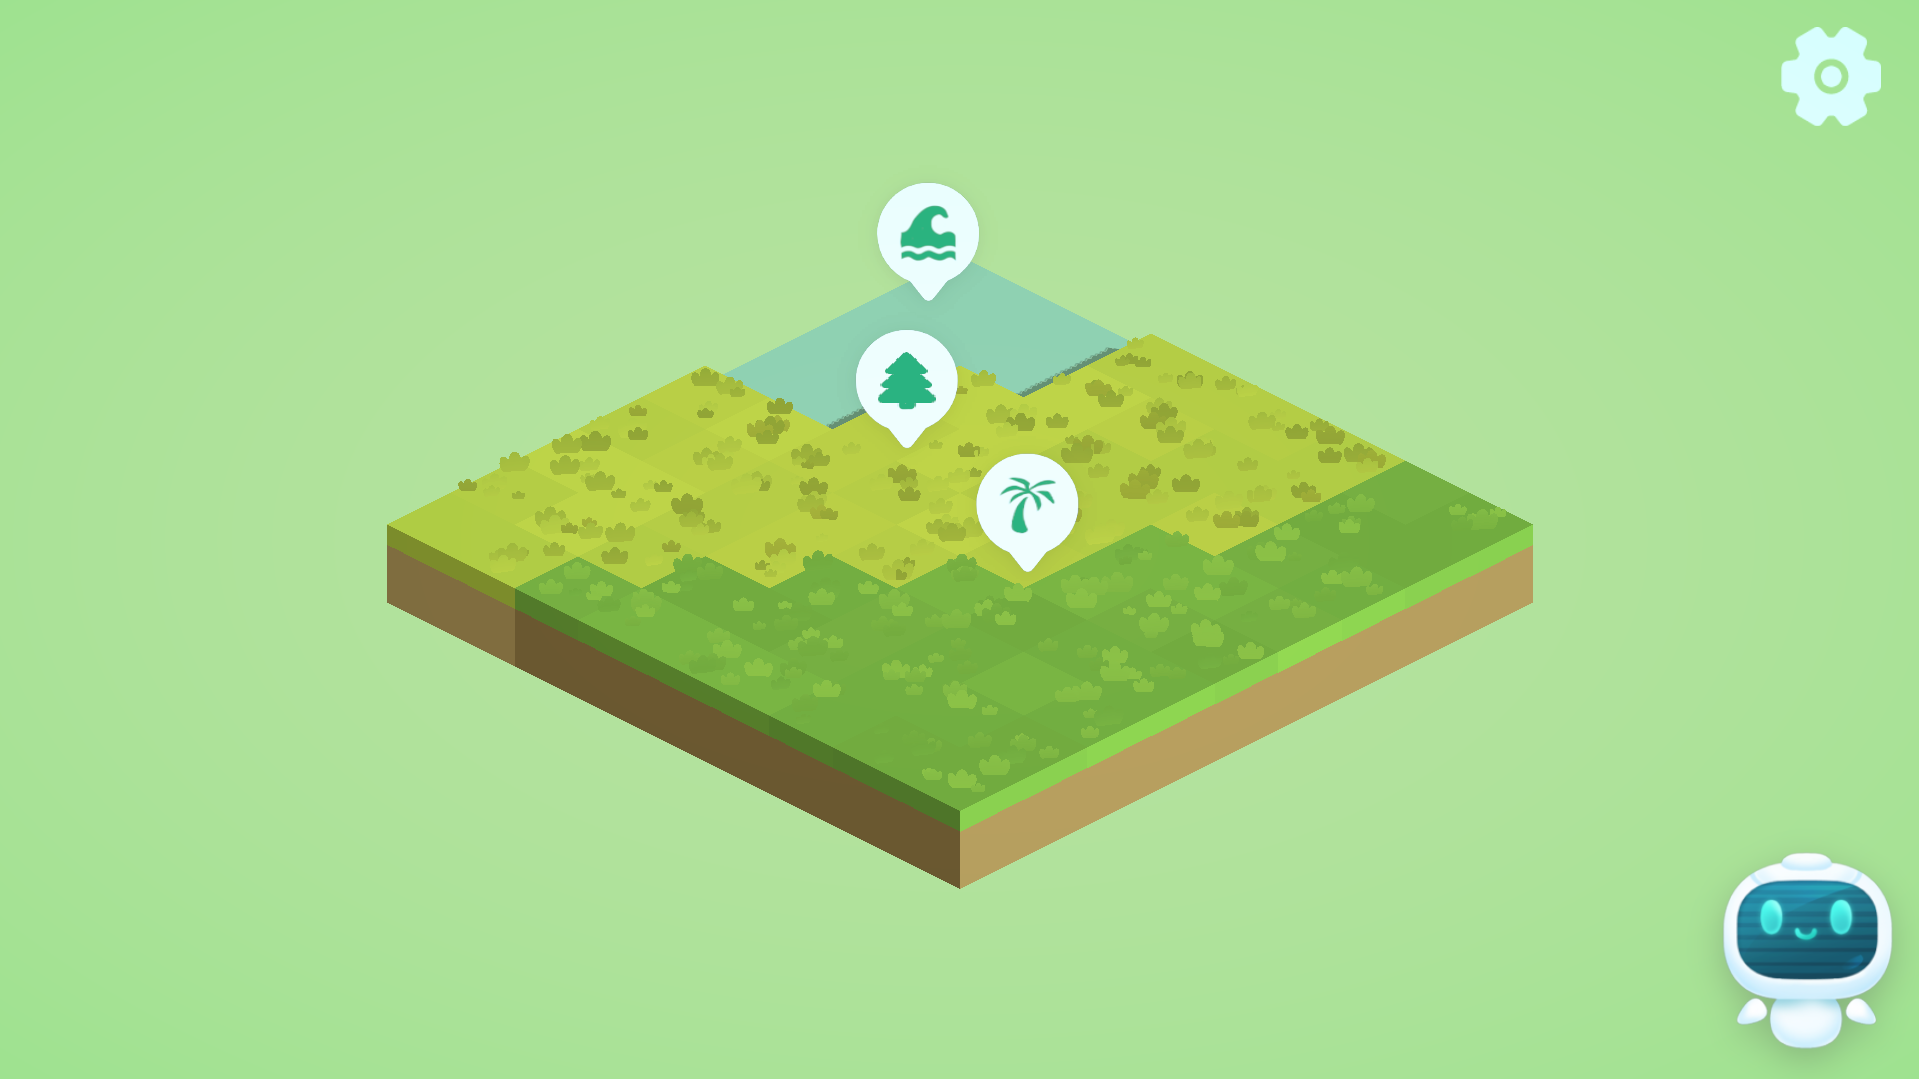
\includegraphics[width=350px,clip=true]{burbujas.png}
  \caption{Mapa con burbujas de bioma visibles}
  \label{fig:burbujas}
\end{figure}

\begin{figure}[H]
  \centering
	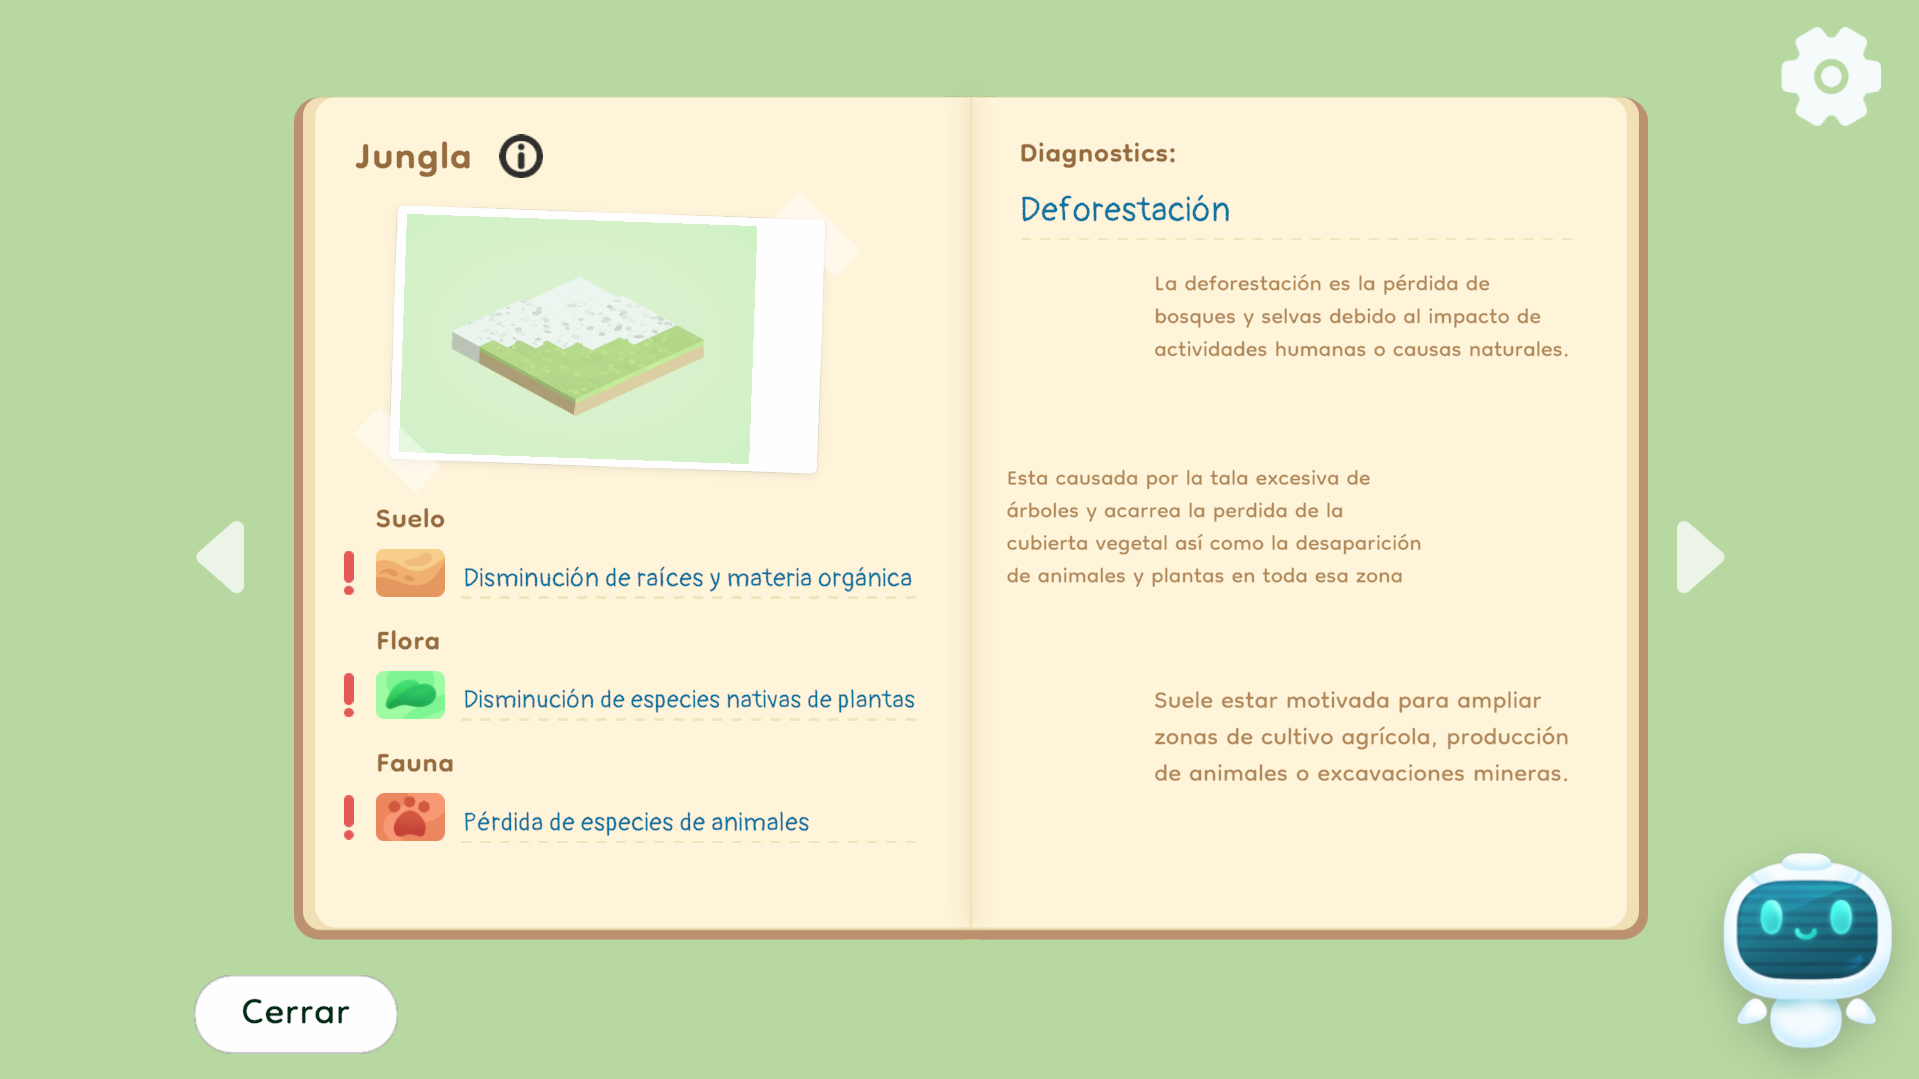
\includegraphics[width=350px,clip=true]{libro_info.png}
  \caption{Libro con información de problemas medioambientales}
  \label{fig:libro}
\end{figure}

\begin{figure}[H]
  \centering
	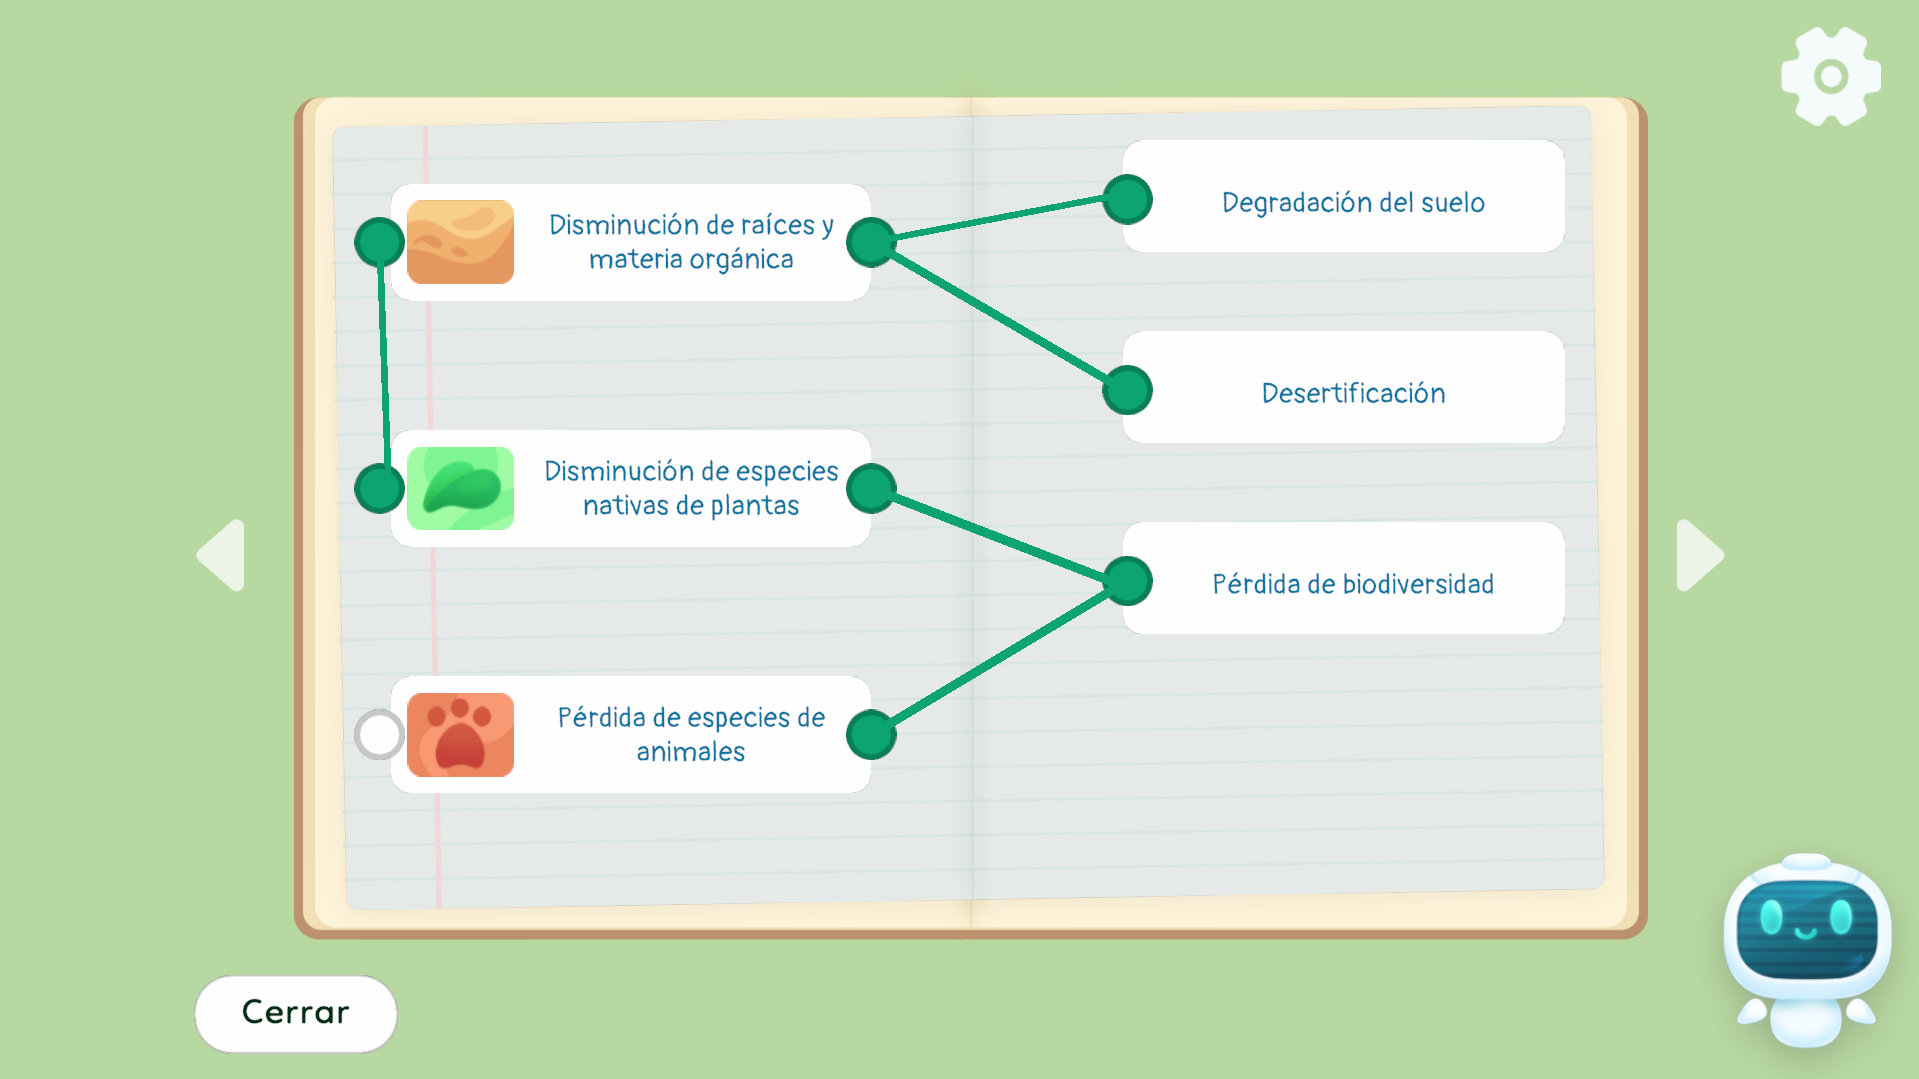
\includegraphics[width=350px,clip=true]{libro_relaciones.png}
  \caption{Libro de Relaciones Problema - Consecuencia}
  \label{fig:relations}
\end{figure}

Una vez el jugador haya demostrado que ha entendido todas las alteraciones y problemas de todos los biomas, el juego pasará a la segunda fase, la de restauración.
\begin{compactitem}
    \item Durante la fase de restauración, el jugador tendrá un presupuesto de energía para gastar en máquinas restauradoras.
    \item Cada bioma tendrá una alteración, que a su vez estará compuesta de 2-3 fases, cada una definida por un problema distinto (Deforestación, Desertificación, Sobrepesca…)
    \item El jugador deberá comprar máquinas restauradoras de la tienda y colocarlas en el bioma para que puedan hacer efecto, los distintos efectos de estas restaurarán el ecosistema de una forma u otra.
    \item La jugabilidad radica en que el jugador tendrá distintas opciones de máquinas (tres) por cada fase de cada bioma, y cada opción tendrá un efecto distinto, teniendo en cuenta la información que ha adquirido durante la primera fase, y la información que proporciona la tienda acerca del efecto de la máquina, el jugador deberá hacer una elección que le permita restaurar el ecosistema por un coste apropiado, con el objetivo de no quedarse sin presupuesto antes de terminar todas las fases de todos los biomas.
\end{compactitem}

Teniendo en cuenta las estrategias del PC y las mecánicas del juego, podemos asimismo definir una tabla (Tabla \ref{fig:tablaPCMecanicas}) que las relacione entre sí, dejando claro de qué forma se pretende ayudar a potenciar el PC en los jugadores.

\raggedbottom
\begin{table}[H]
\begin{center}
\setlength{\tabcolsep}{5pt}
\renewcommand{\arraystretch}{1.2}
\begin{tabular}{ | m{8em} | m{30em} | } 
  \hline
  Estrategia & Mecánica \\ 
  \hline
  Abstracción & A la hora de realizar los diagramas de correlación entre indicadores (datos) y sus consecuencias, se reduce al mínimo imprescindible la explicación del contexto de la alteración del ecosistema. \\ 
  \hline
  Análisis de Datos & La fase de investigación muestra una serie de datos que posteriormente el jugador analiza para poder correlacionarlos con consecuencias. \\ 
  \hline
  Descomposición de problemas & Un nivel está visiblemente desglosado en diferentes tareas y subtareas. Para completar el nivel es necesario restaurar todos los biomas y para restaurar cada bioma hay que finalizar todas las fases del plan de restauración (que pueden considerarse tareas a cumplimentar). \\ 
  \hline
  Algoritmia & A la hora de restaurar un ecosistema, está todo claramente separado de forma secuencial. Incluso el propio nivel se desarrolla de forma secuencial. \\ 
  \hline
  Depuración de Errores & Es posible cometer errores y es importante detectarlos y subsanarlos a tiempo. La idea es dejar cierto margen para que los jugadores puedan echarse atrás y arreglar los fallos. \\ 
  \hline
    & El jugador tiene recursos (moneda) limitados y debe hacer un buen uso de ellos para poder completar los niveles, si se queda sin dinero, deberá volver a intentarlo para poder minimizar el gasto. \\ 
  \hline
  Generalización & A menudo las alteraciones de los ecosistemas tienen factores en común, a lo largo del progreso en el videojuego los jugadores podrán ir discerniendo que existen muchas correlaciones entre alteraciones y sus consecuencias. Por ejemplo: Si hay un problema con el suelo (del tipo que sea) la flora no va a poder prosperar correctamente y si la flora no está en sus condiciones óptimas, la fauna tampoco lo estará. \\ 
  \hline
\end{tabular}
\centering
\caption{Relaciones entre Estrategias del PC con mecánicas del videojuego.}
\label{fig:tablaPCMecanicas}
\end{center}
\end{table}

\section{Motivación}

La motivación para el desarrollo de EcoRescue nace como respuesta al Plan de Acción de Educación Digital 2021-2027 de la Comisión Europea\cite{europaPlan}, además de verse reforzada en 
España por la modificación de la Ley Orgánica 3/2020 del 3 de diciembre de 2020\cite{lomce}, y los Reales Decretos 95/2022\cite{boeInfantil}, 157/2022\cite{boePrimaria}, 217/2022\cite{boeSecundaria} y 243/2022\cite{boebachillerato}, del 1 de febrero, 1 y 19 de marzo y 5 de abril del 2022 respectivamente, 
que establecen las enseñanzas mínimas de la educación, incluyendo el PC, en las etapas de Educación Infantil, Primaria y Secundaria Obligatoria y Bachillerato, como una competencia transversal en diversas asignaturas o en asignaturas determinadas.

Como se ha mencionado anteriormente, además de servir para desarrollar el PC, uno de los objetivos del proyecto es concienciar sobre la importancia de cuidar el medioambiente y de como distintos indicadores y alteraciones pueden afectar negativamente a estos. De esta forma, el juego puede ayudar a niños y adolescentes a relacionar consecuencias del sistema productivo de la sociedad actual con los daños que sufren actualmente nuestros ecosistemas y entornos naturales. A su vez, ilustra de forma eficiente como interaccionan diferentes ecosistemas entre sí y como se relacionan sus diferentes elementos: fauna, flora y el soporte natural. Además, el juego aporta una versión optimista de como entornos que se consideran destruidos se pueden recuperar mediante la intervención y tecnología adecuados. 

Este enfoque es relevante dado que según los Reales Decretos mencionados anteriormente\cite{boeInfantil}\cite{boePrimaria}\cite{boeSecundaria}\cite{boebachillerato} se estipula que en lo relacionado al Conocimiento del Medio, Biología y Geología se buscará fomentar el razonamiento y pensamiento crítico (computacional) para resolver problemas o dar explicación a procesos de la vida cotidiana.

Finalmente habría que considerar también la motivación adicional de aprender el uso de nuevas tecnologías mediante el desarrollo de un proyecto, que tendría como objetivo el propio aprendizaje y la acumulación de experiencia de llevar un proyecto desde su etapa de concepción hasta validarlo con un grupo de alumnos de instituto.

\raggedbottom
\section{Objetivos}
\subsection{Objetivos generales}
El objetivo general del trabajo es la elaboración de un prototipo funcional del videojuego EcoRescue para el desarrollo del PC y la concienciación en la restauración de ecosistemas, 
en el que los jugadores puedan acceder a niveles generados procedimentalmente, compuestos por un número
de 1-N biomas. Posteriormente deberán poder informarse de estos, relacionar problemas y consecuencias (Figura \ref{fig:diagconsecuencias}) y finalmente 
colocar máquinas en los biomas para restaurar los distintos problemas de cada alteracion.

\begin{figure}[H]
  \centering
    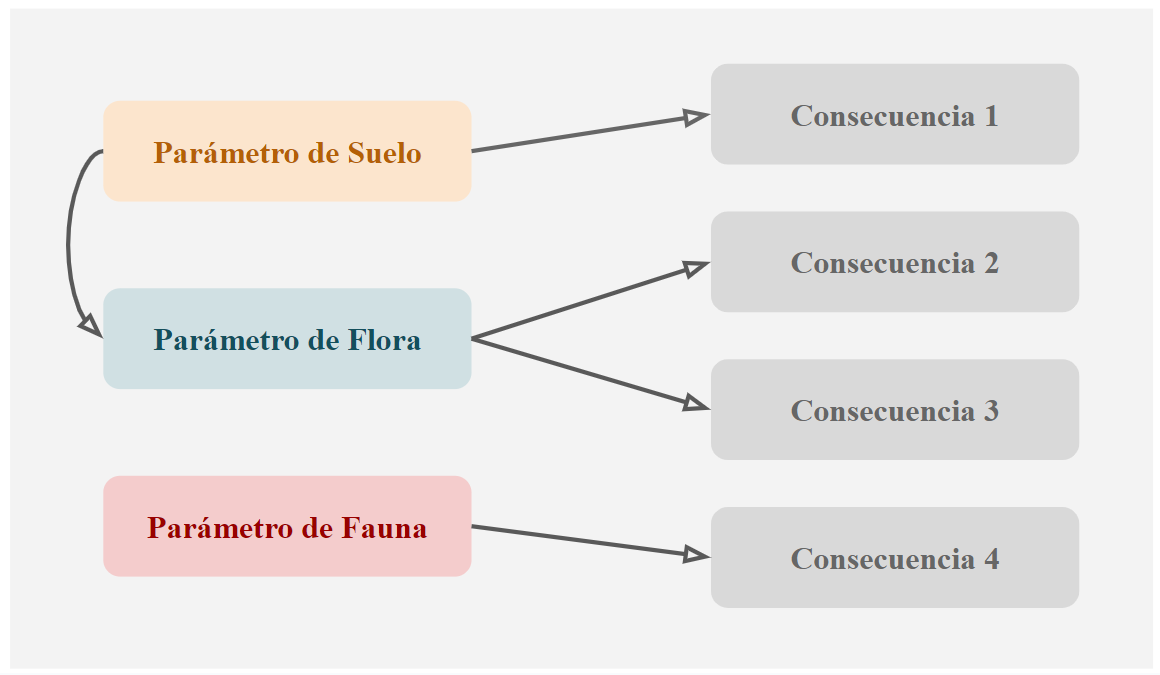
\includegraphics[width=350px,clip=true]{diagramaproblemasconsecuencias.png}
  \caption{Diagrama de relaciones entre problemas y problemas y consecuencias}
  \label{fig:diagconsecuencias}
\end{figure}

El prototipo deberá tener interfaces funcionales que muestren la información de los niveles, biomas, alteraciones, problemas, consecuencias, máquinas y tutoriales (Figuras \ref{fig:UI} y \ref{fig:diagUI}). Los tutoriales vendrán dados por diálogos que saldrán del 
icono de un robot (Figura \ref{fig:robot}) que guiará al jugador durante su experiencia de juego.

\begin{figure}[H]
    \centering
      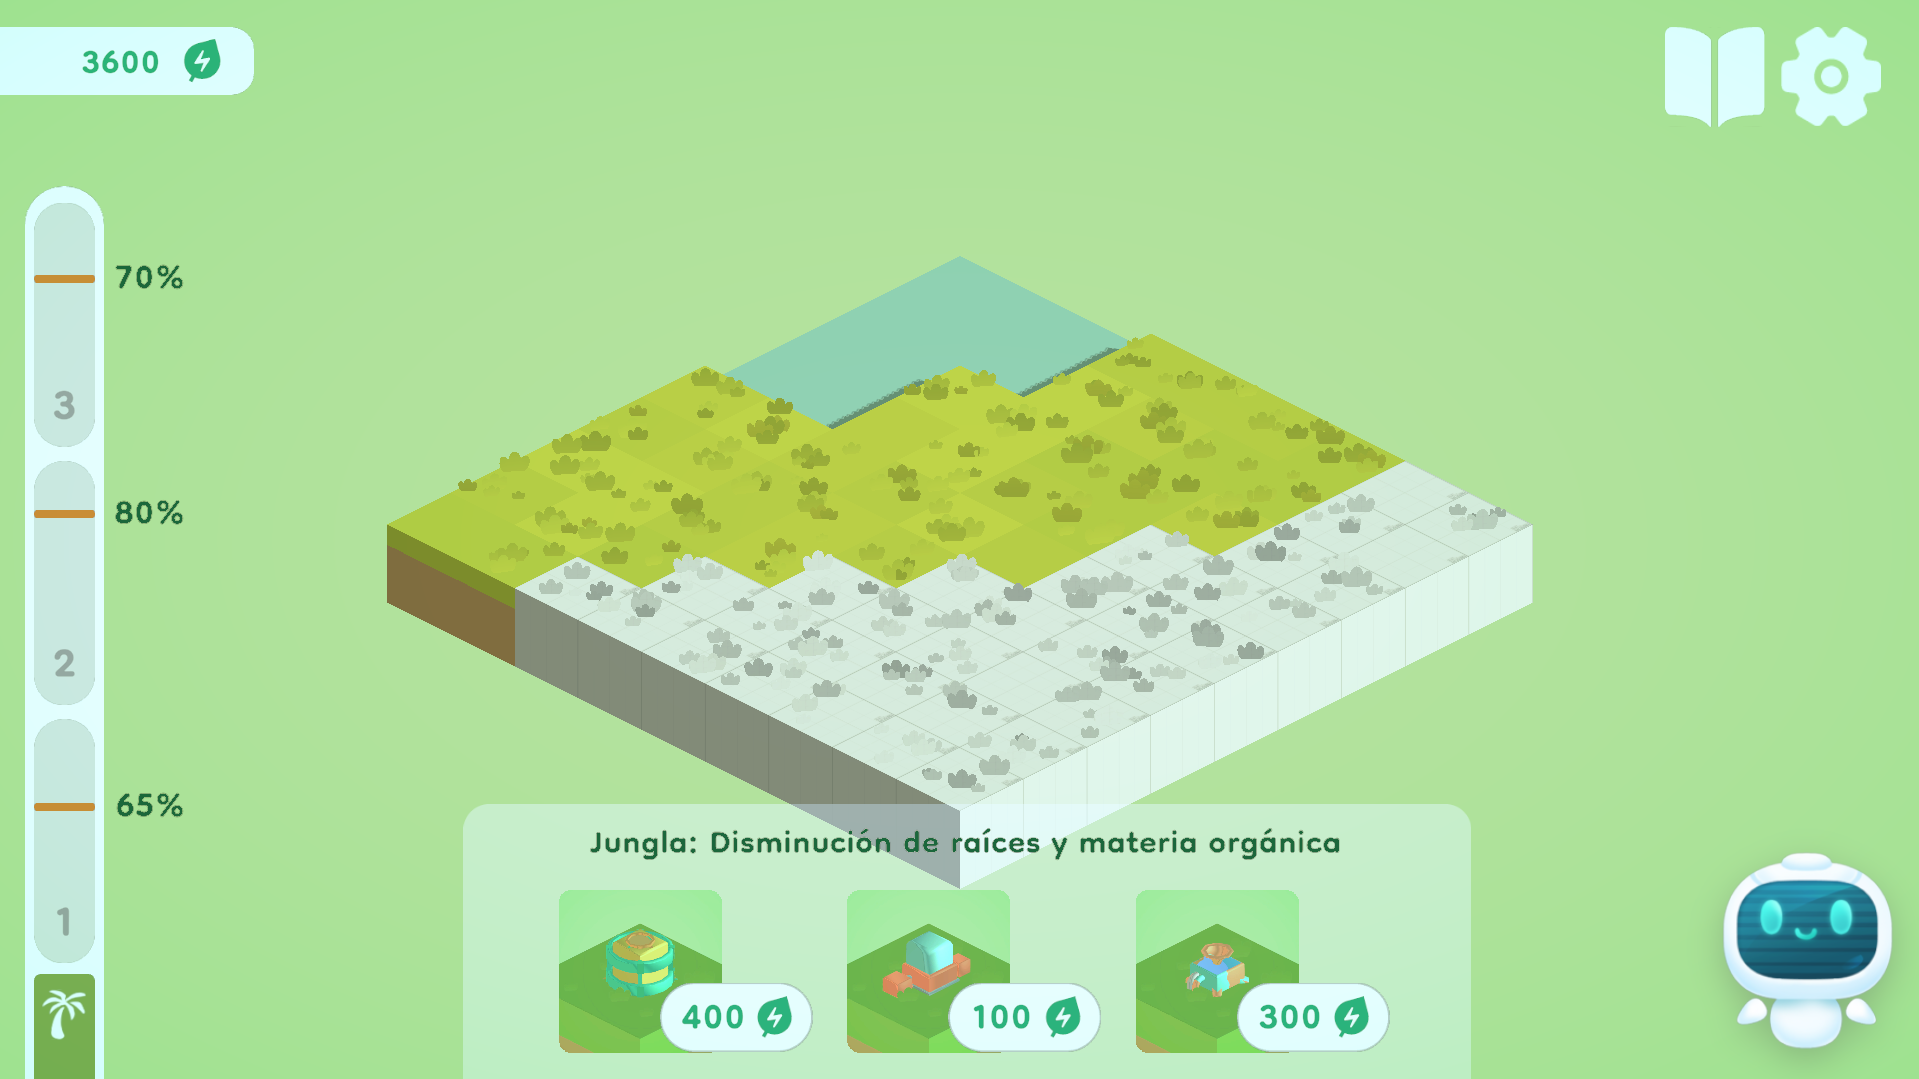
\includegraphics[width=350px,clip=true]{interfaz_restauracion.png}
    \caption{Interfaz general de EcoRescue}
    \label{fig:UI}
\end{figure}

\begin{figure}[H]
    \centering
      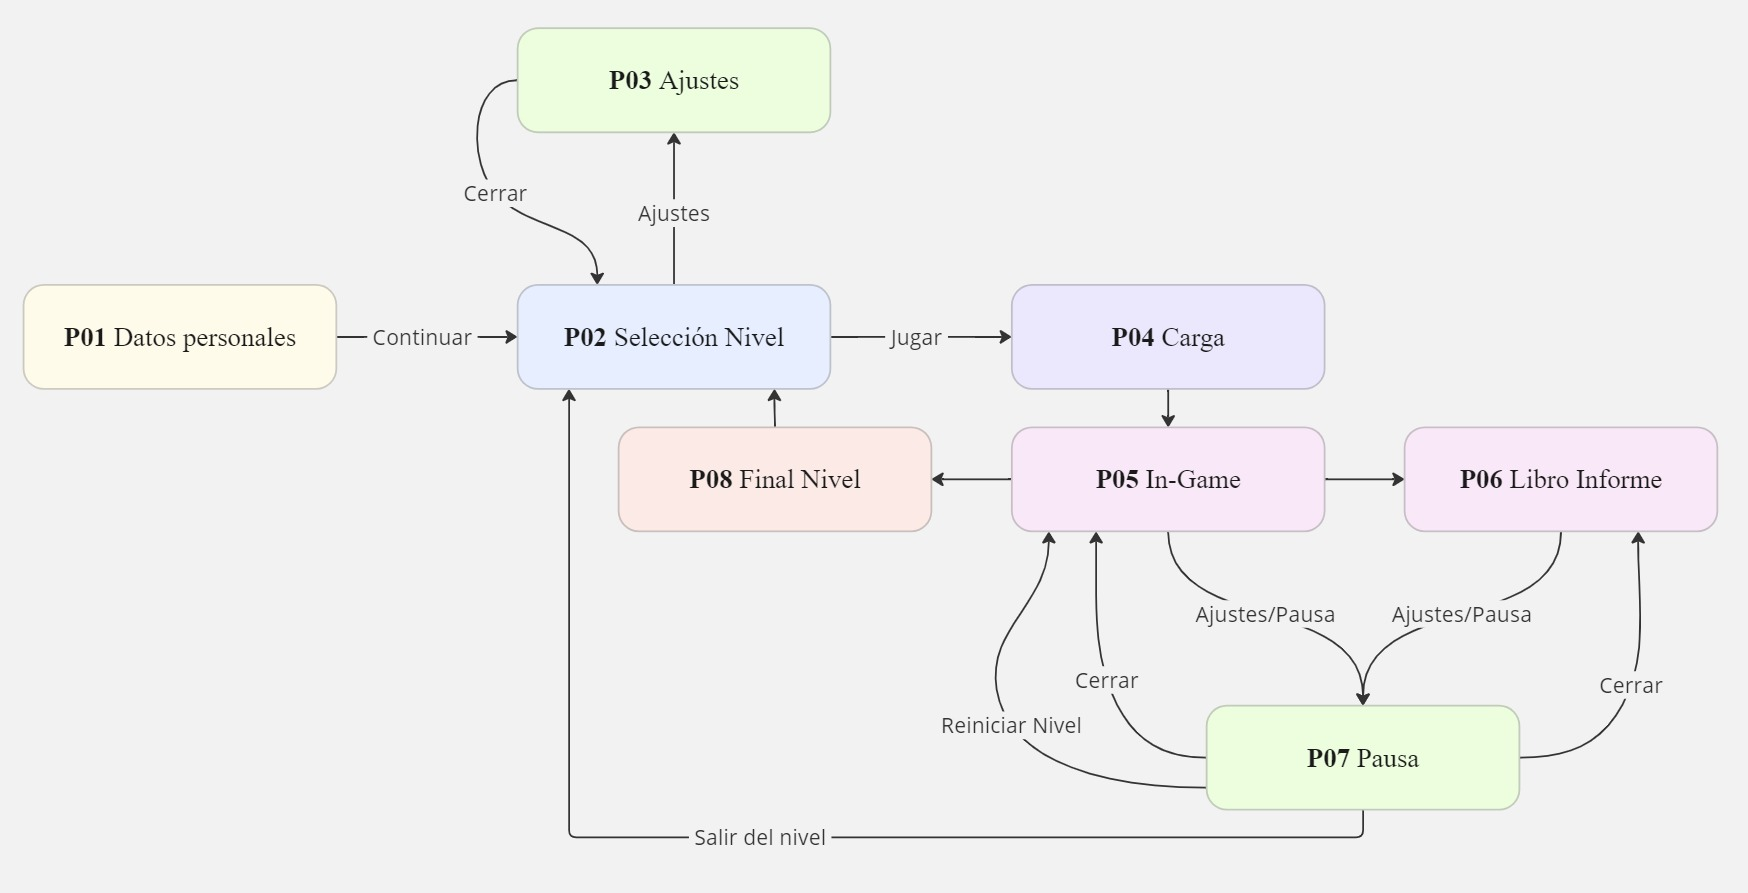
\includegraphics[width=350px,clip=true]{diagramapantallas.jpg}
    \caption{Diagrama de flujo de UI de EcoRescue}
    \label{fig:diagUI}
\end{figure}

\begin{figure}[H]
    \centering
      
\includegraphics[width=350px,clip=true]{convo_robot.png}
    \caption{Conversación de tutorial del robot}
    \label{fig:robot}
\end{figure}

El prototipo también deberá ser jugablemente disfrutable, esto implica desarrollar sistemas de control, sonido y animaciones que hagan que el juego sea vistoso y satisfactorio de jugar.

\subsection{Generación procedimental}

Una parte importante de EcoRescue es la facilidad de creación de contenido, para que desarrollar niveles sea más sencillo, el juego se ha enfocado desde un principio con la generación procedimental en mente, de forma que los niveles deberán generarse en base a algoritmia\cite{FastNoiseLite}, y cosas como las alteraciones en un nivel o el percentil (Figura \ref{fig:percentil}) al que se debe completar una fase deberán del mismo modo seguir un patrón procedimental.

\begin{figure}[H]
  \centering
    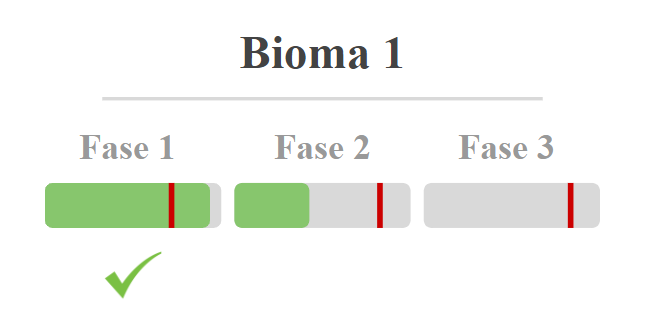
\includegraphics[width=350px,clip=true]{diagramafases.png}
  \caption{Diagrama explicativo de los percentiles a completar de cada fase}
  \label{fig:percentil}
\end{figure}

\subsection{Herramientas del desarrollo}

De cara a la generación procedimental de niveles, el prototipo necesitará herramientas para que enlazar el gran volumen de contenido requerido por este enfoque de desarrollo con las estructuras internas del videojuego sea sencillo y mayormente automatizado. 

De esta forma, se requiere desarrollar un script que importe automáticamente todo el contenido (biomas, alteraciones, problemas, consecuencias, sprites, modelos...) desde un fichero de excel a un formato legible por el juego.

Además, también se requiere la creación de herramientas que permitan elegir de qué forma se quiere que se presente un nivel, incluyendo: personalización de las reglas de la generación procedimental de mapas, selección de Biomas por nivel y selección de Alteraciones por Bioma.

Además, el prototipo necesitará un sistema de generación de diálogos para que el robot de los tutoriales pueda comunicarse efectivamente con el jugador.

\subsection{Recogida de datos}

De cara a la medición de resultados, es necesario que el prototipo sea capaz de comunicarse con una base de datos para poder monitorizar las partidas de los jugadores y así poder interpretar sus movimientos. 
Esta comunicación con la base de datos debería recoger los datos básicos del usuario (nombre, edad...) (Figura \ref{fig:datos}) así como datos sobre su partida (máquinas colocadas, relaciones correctas, veces que ha perdido el nivel...).

\begin{figure}[H]
    \centering
      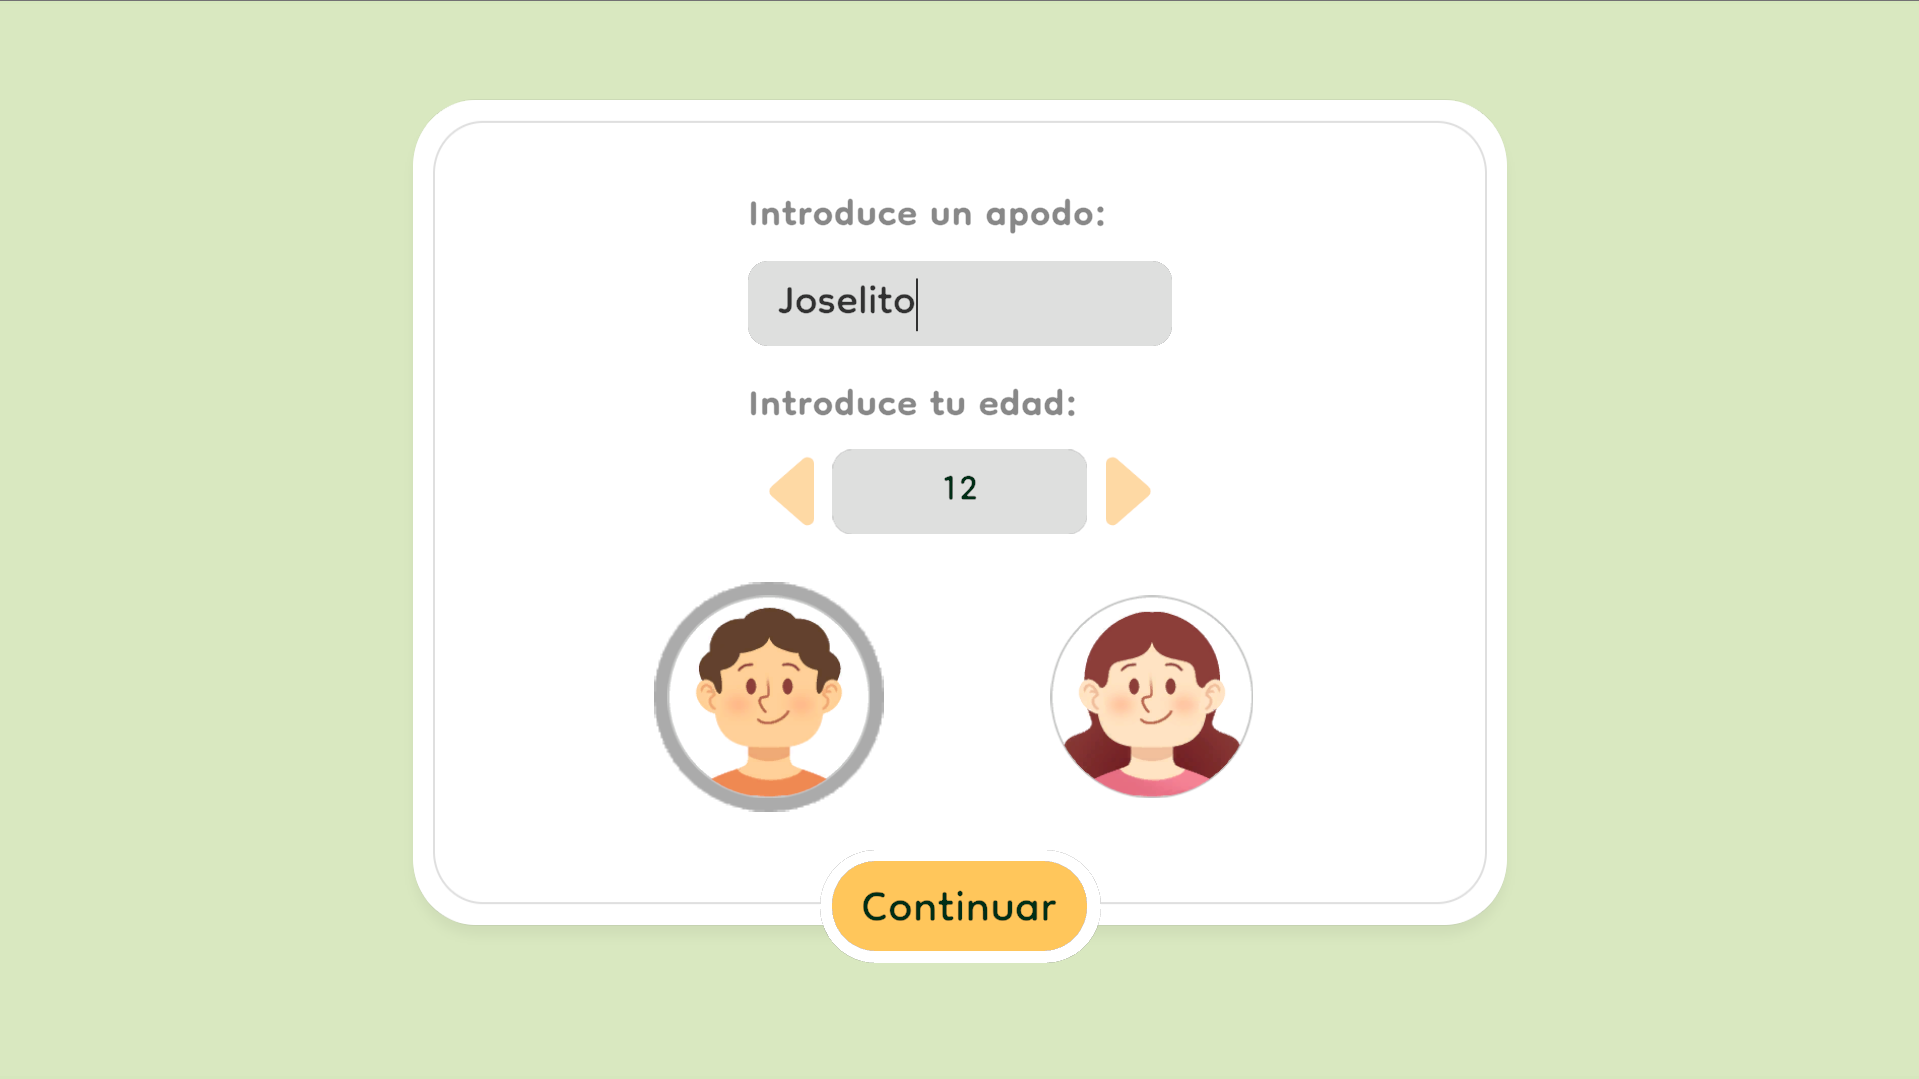
\includegraphics[width=350px,clip=true]{datos_pj.png}
    \caption{Pantalla de introducción de datos personales}
    \label{fig:datos}
\end{figure}

\subsection{Validación}

El objetivo más importante a nivel de proyecto es validar el prototipo frente a un grupo de alumnos de 1º de la ESO reales, con el objetivo de poder utilizar los datos de una encuesta así como los datos obtenidos en la base de datos para poder extraer conclusiones acerca de la efectividad del prototipo como herramienta didáctica para el desarrollo del PC, además de como herramienta divulgativa en lo referente a la restauración de ecosistemas.
Queda patente, pues, que los objetivos de la validación deben ser:
\begin{compactitem}
    \item Que el juego verdaderamente sirva para desarrolar el PC.
    \item Que el juego divulge información interesante acerca de la restauración de ecosistemas.
    \item Que el juego resulte una expriencia amena y divertida, a fin de que los alumnos disfruten del aprendizaje.
\end{compactitem} 

\subsection{Resumen de Objetivos}

En resumen, el el proyecto pretende, como objetivo principal desarrollar un juego completo y funcional que permita al jugador informarse sobre la restauración de ecosistemas y actuar en consecuencia.

Además de los objetivos secundarios:
\begin{compactitem}
  \item Desarrollar el PC del jugador en el aula.
  \item Desarrollar un juego que sea divertido y ameno.
  \item Desarrollar un juego con niveles generados procedimentalmente, además de herramientas que permitan crear contenido de forma eficiente para este.
  \item Recabar información sobre las partidas de los jugadores con el objetivo de interpretar sus movimientos y extraer conclusiones sobre la efectividad del prototipo.
\end{compactitem}

\section{Metodología}

Para el desarrollo del prototipo se ha utilizado una metodología de trabajo iterativa-incremental enfocada en la revisión de objetivos y
avances entre el tutor y los alumnos. Durante una serie de revisiones se ha evaluado el estado del proyecto y se han marcado objetivos de cara a las siguientes revisiones. El desarrollo se puede dividir en tres fases: 
\begin{itemize}
	\item Fase 1: Pre-Producción y Análisis de Requisitos, Junio 2023 - Diciembre 2023
	\item Fase 2: Producción, Enero 2024 - Mayo 2024
	\item Fase 3: Polish y Validación, Junio 2024 
\end{itemize}

La primera fase se utilizó como una ventana de tiempo en la que prototipar los controles y la generación procedimental del mapa, además de realizar un análisis de requisitos y un documento de diseño exhaustivo para tener claro qué clase de prototipo realizar. Este documento de diseño se fue iterando con \nombretutor de cara a la producción final.

Durante la segunda fase se realizó el groso de la producción del juego, con el diseño ya fijado, esta fase consistió sobre todo en implementar el bucle de juego general y definir el contenido que iba a estar presente en el juego final.

La tercera y última fase consistió en la creación de herramientas para el desarrollo de contenido/niveles, pulir el juego añadiendo pequeñas animaciones, efectos y sonidos, implementar un sistema de recogida de datos en tiempo real via una base de datos remota y finalmente acudir a un instituto para poder validar el prototipo con alumnos de verdad.

En adelante se detalla el plan de producción.

\subsection{Fase 1: Pre-Producción y Análisis de Requisitos (Junio 2023 - Diciembre 2023))}

Figura \ref{fig:fase1gantt}.

\subsubsection{Primer Hito (25 de junio)}
\begin{compactitem}
\item F1T1: Análisis de requisitos (Marta y Ángel) (1 de junio - 7 de junio)
\item F1T2: Propuesta de concepto inicial (Marta y Ángel) (8 de junio - 21 de junio)
\end{compactitem}
Iteraciones de Prototipos (4 ciclos de 4 semanas cada uno)

\subsubsection{Segundo Hito (9 de julio) Prototipo 1}

\begin{compactitem}
  \item F1P1T3: Planificación del prototipo (Marta y Ángel) (22 de junio - 28 de junio)
  \item F1P1T4: Desarrollo de arte/diseño (Marta) (29 de junio - 12 de julio)
  \item F1P1T5: Desarrollo de programación (Ángel) (29 de junio - 19 de julio)
  \item F1P1T6: Avance de concept art/contenido diseño (Marta) (13 de julio - 19 de julio)
\end{compactitem}

\subsubsection{Tercer Hito (6 de agosto) Prototipo 2}

\begin{compactitem}
  \item F1P2T1: Planificación del prototipo (Marta y Ángel) (20 de julio - 26 de julio)
  \item F1P2T2: Desarrollo de arte/diseño (Marta) (27 de julio - 9 de agosto)
  \item F1P2T3: Desarrollo de programación (Ángel) (27 de julio - 16 de agosto)
  \item F1P2T4: Avance de concept art/contenido diseño (Marta) (10 de agosto - 16 de agosto)
\end{compactitem}

\subsubsection{Cuarto Hito (3 de septiembre) Prototipo 3}

\begin{compactitem}
\item F1P3T1: Planificación del prototipo (Marta y Ángel) (17 de agosto - 23 de agosto)
\item F1P3T2: Desarrollo de arte/diseño (Marta) (24 de agosto - 6 de septiembre)
\item F1P3T3: Desarrollo de programación (Ángel) (24 de agosto - 13 de septiembre)
\item F1P3T4: Avance de concept art/contenido diseño (Marta) (7 de septiembre - 13 de septiembre)
\end{compactitem}


\subsubsection{Quinto Hito (1 de octubre) Prototipo 4}

\begin{compactitem}
\item F1P4T1: Planificación del prototipo (Marta y Ángel) (14 de septiembre - 20 de septiembre)
\item F1P4T2: Desarrollo de arte/diseño (Marta) (21 de septiembre - 4 de octubre)
\item F1P4T3: Desarrollo de programación (Ángel) (21 de septiembre - 11 de octubre)
\item F1P4T4: Avance de concept art/contenido diseño (Marta) (5 de octubre - 11 de octubre)
\end{compactitem}


\subsubsection{Sexto Hito (10 de diciembre) Documentación y Planificación}

\begin{compactitem}
\item F1T4: Elaboración del documento de diseño (Marta y Ángel) (12 de octubre - 10 de diciembre)
\item F1T5: Planificación del código (Ángel) (12 de octubre - 10 de diciembre)
\item F1T6: Avance de concept art y diseño de un prototipo de baja fidelidad UI/UX (Marta) (12 de octubre - 10 de diciembre)
\end{compactitem}

\begin{figure}[H]
  \centering
	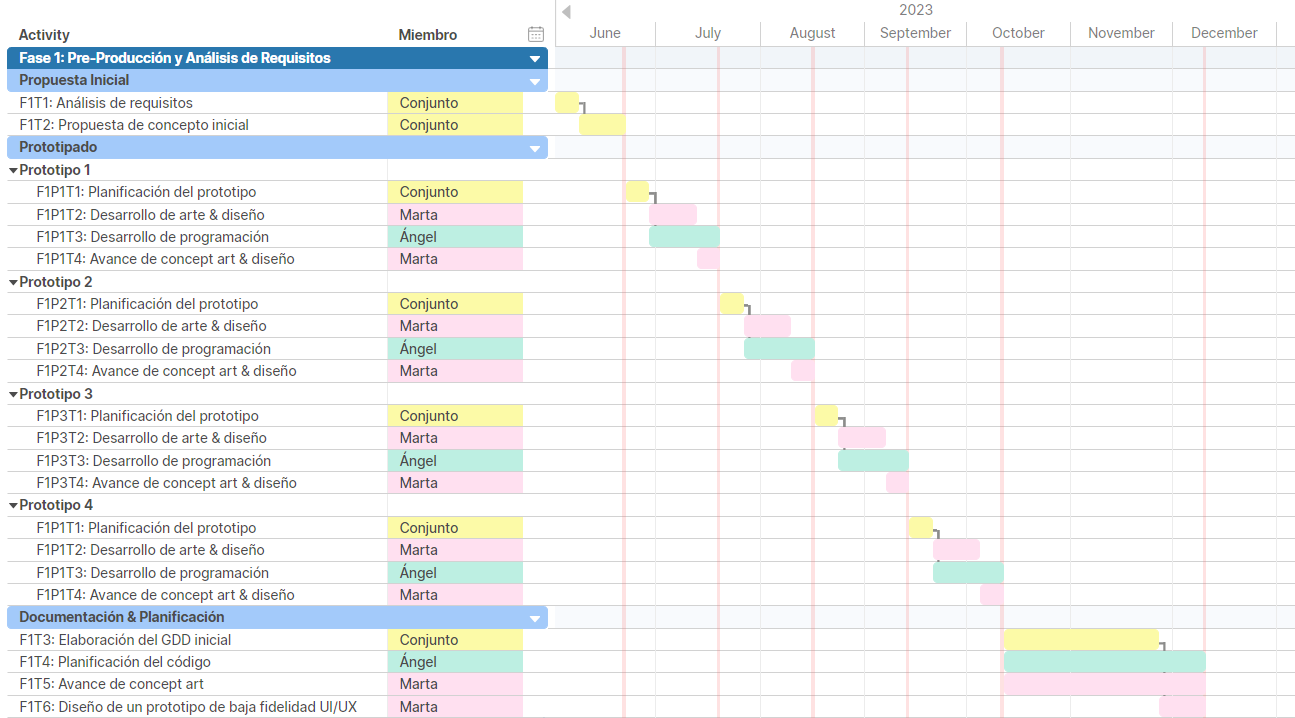
\includegraphics[width=350px,clip=true]{gantt1.png}
  \caption{Diagrama de Gantt de la fase 1 de producción}
  \label{fig:fase1gantt}
\end{figure}

\subsection{Fase 2: Producción (Enero 2024 - Mayo 2024)}

Figura \ref{fig:fase2gantt}.

\subsubsection{Primer Hito (17 de marzo)}

\begin{compactitem}
\item F2T1: Generación de un mapa y sistema de máquinas (Ángel) (21 de enero - 10 de marzo)
\item F2T2: Escenario 3D y paleta de colores (Marta) (21 de enero - 11 de febrero)
\item F2T3: Versión funcional del prototipo de alta fidelidad UI/UX (Marta) (12 de febrero - 25 de febrero)
\item F2T4: Redacción de contenido para los 3 biomas iniciales (Marta) (12 de febrero - 17 de marzo)
\item F2T5: Implementar arte (Ángel) (11 de marzo - 17 de marzo)
\end{compactitem}

\subsubsection{Segundo Hito (21 de abril)}

\begin{compactitem}
\item F2T6: Sistema de niveles y generación procedimental (Ángel) (18 de marzo - 21 de abril)
\item F2T7: Sistemas de objetivos y recursos (Ángel) (18 de marzo - 21 de abril)
\item F2T8: Redacción de contenido y parámetros de diseño para las máquinas (Marta) (18 de marzo - 24 de marzo)
\item F2T9: Modelos 3D para las máquinas (Marta) (25 de marzo - 31 de marzo)
\item F2T10: Prototipo de alta fidelidad casi final (Marta) (1 de abril - 11 de abril)
\item F2T11: Implementar interfaz esencial (Ángel) (11 de abril - 21 de abril)
\end{compactitem}

\subsubsection{Tercer Hito (26 de mayo)}

\begin{compactitem}
\item F2T12: Assets finales de la interfaz (Marta) (22 de abril - 9 de mayo)
\item F2T13: Pulido de bugs (Ángel) (22 de abril - 26 de abril)
\item F2T14: Revisión de contenido y balanceo final de las máquinas (Marta) (10 de mayo - 19 de mayo)
\item F2T15: Implementación del sistema del libro de informes y minijuegos (Ángel) (27 de abril - 19 de mayo)
\item F2T16: Implementación de la interfaz final (Ángel) (20 de mayo - 26 de mayo)
\item F2T17: Ilustraciones decorativas esenciales (Marta) (20 de mayo - 25 de mayo)
\item F2T18: Implementación ilustraciones decorativas esenciales (Ángel) (26 de mayo)
\end{compactitem}

\begin{figure}[H]
  \centering
	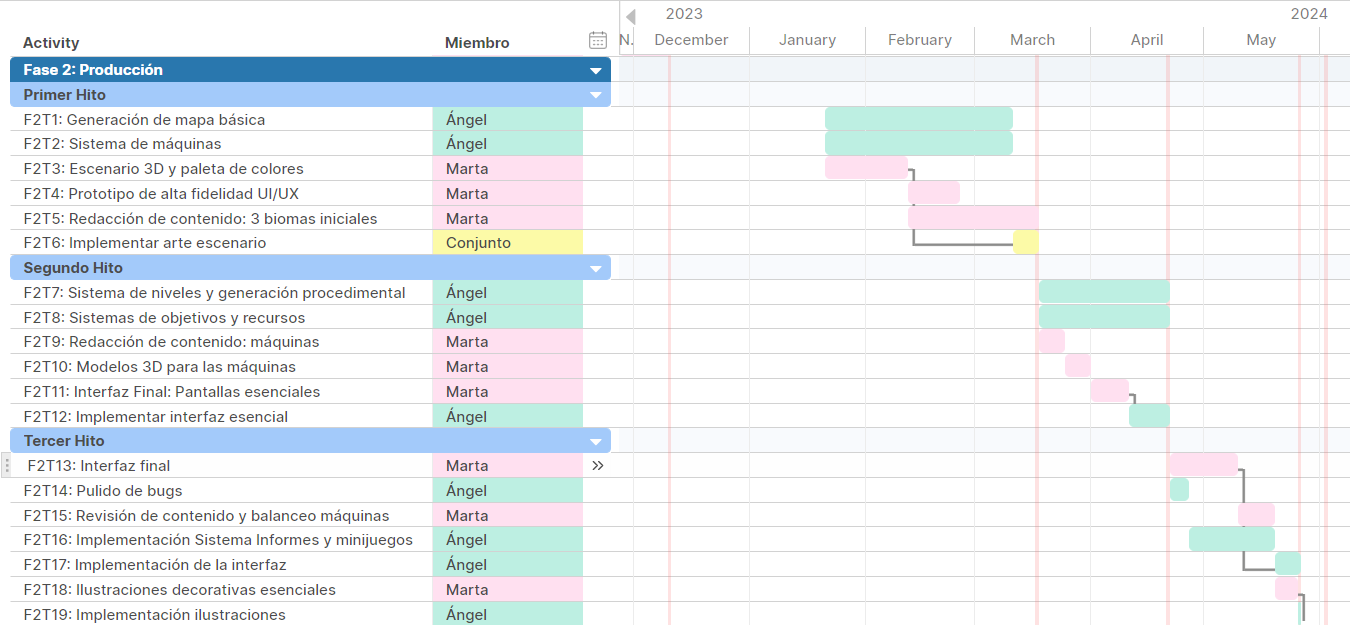
\includegraphics[width=350px,clip=true]{gantt2.png}
  \caption{Diagrama de Gantt de la fase 2 de producción}
  \label{fig:fase2gantt}
\end{figure}

\subsection{Fase 3: Polish y Validación (Junio 2024)}

Figura \ref{fig:fase3gantt}.

\subsubsection{Primer Hito (2 de junio)}

\begin{compactitem}
\item F3T1: Creación de herramientas para el desarrollo de contenido/niveles (Ángel) (27 de mayo - 2 de junio)
\item F3T2: Retoques de balanceo y contenido (Marta) (27 de mayo - 2 de junio)
\end{compactitem}

\subsubsection{Segundo Hito (9 de junio)}

\begin{compactitem}
\item F3T3: Añadir pequeñas animaciones, efectos y sonidos (Marta y Ángel) (2 de junio - 9 de junio)
\item F3T4: Implementación de sistema de recogida de datos en tiempo real (Ángel) (2 de junio - 9 de junio)
\end{compactitem}

\subsubsection{Tercer Hito (13 de junio)}

\begin{compactitem}
  \item F3T5: Últimos retoques (Marta y Ángel) (10 de junio - 13 de junio)
\end{compactitem}

\begin{figure}[H]
  \centering
	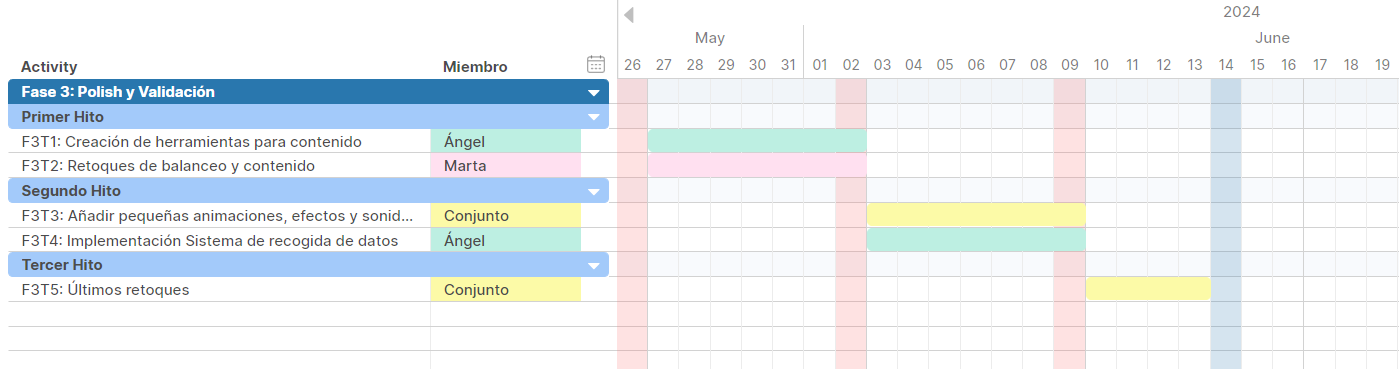
\includegraphics[width=350px,clip=true]{gantt3.png}
  \caption{Diagrama de Gantt de la fase 3 de producción}
  \label{fig:fase3gantt}
\end{figure}

Esta metodología ha acabado siendo todo un exito con este prototipo, ya que ha permitido un avance progresivo donde no ha acabado habiendo esfuerzo malgastado, esto ha permitido que el desarrollo del prototipo haya sido sólido y no se hayan requerido cambios radicales.

% \afterpage{\blankpage} % puede generar problema en índice de contenidos
% \newpage


% Capítulo 2
\chapter{Objetivos}
\section*{Objetivos generales}
El objetivo general del trabajo es la elaboración de un prototipo funcional del videojuego EcoRescue, en el que los jugadores puedan acceder a niveles generados procedimentalmente, compuestos por un número de 1-N biomas y de 1-3 alteraciones. Posteriormente deberán poder informarse de estos, relacionar alteraciones y consecuencias y finalmente colocar máquinas en los biomas para restaurar las distintas alteraciones.

El prototipo deberá tener interfaces funcionales que muestren la información de los niveles, biomas, alteraciones, máquinas y tutoriales. Los tutoriales vendrán dados por diálogos que saldrán del 
icono de un robot que guiará al jugador durante su experiencia de juego.

El prototipo también deberá ser jugablemente disfrutable, esto implica desarrollar sistemas de control, sonido y animaciones que hagan que el juego sea vistoso y satisfactorio de jugar.

\section*{Generación procedimental}

Una parte importante de EcoRescue es la facilidad de creación de contenido, para que desarrollar niveles sea más sencillo, el juego se ha enfocado desde un principio con la generación procedimental en mente, de forma que los niveles deberán generarse en base a algoritmia\cite{FastNoiseLite}, y cosas como las alteraciones en un nivel o el percentil al que se debe completar una fase deberán del mismo modo seguir un patrón procedimental.

\section*{Herramientas del desarrollo}

De cara a la generación procedimental de niveles, el prototipo necesitará herramientas para que enlazar el gran volumen de contenido requerido por este enfoque de desarrollo con las estructuras internas del videojuego sea sencillo y mayormente automatizado. 

De esta forma, se requiere desarrollar un script que importe automáticamente todo el contenido (biomas, alteraciones, consecuencias, sprites, modelos...) desde un fichero de excel a un formato legible por el juego.

Además, también se requiere la creación de herramientas que permitan elegir de qué forma se quiere que se presente un nivel, incluyendo: personalización de las reglas de la generación procedimental de mapas, selección de Biomas por nivel y selección de Alteraciones por Bioma.

Además, el prototipo necesitará un sistema de generación de diálogos para que el robot de los tutoriales pueda comunicarse efectivamente con el jugador.

\section*{Recogida de datos}

De cara a la medición de resultados, es necesario que el prototipo sea capaz de comunicarse con una base de datos para poder monitorizar las partidas de los jugadores y así poder interpretar sus movimientos. 
Esta comunicación con la base de datos debería recoger los datos básico  del usuario (nombre, edad...) así como datos sobre su partida (máquinas colocadas, relaciones correctas, veces que ha perdido el nivel...).

\section*{Validación}

El objetivo más importante a nivel de proyecto es validar el prototipo frente a un grupo de alumnos de 1º de la ESO reales, con el objetivo de poder utilizar los datos de una encuesta así como los datos obtenidos en la base de datos para poder extraer conclusiones acerca de la efectividad del prototipo como herramienta didáctica para el desarrollo del PC, además de como herramienta divulgativa en lo referente a la restauración de ecosistemas.
Queda patente, pues, que los objetivos de la validación deben ser:
\begin{compactitem}
    \item Que el juego verdaderamente sirva para desarrolar el PC.
    \item Que el juego divulge información interesante acerca de la restauración de ecosistemas.
    \item Que el juego resulte una expriencia amena y divertida, a fin de que los alumnos disfruten del aprendizaje.
\end{compactitem} 

\section*{Resumen de Objetivos}

En resumen, el el proyecto pretende:
\begin{enumerate}
    \item Desarrollar un juego completo y funcional que permita al jugador informarse sobre la restauración de ecosistemas y actuar en consecuencia.
    \item Desarrollar el PC del jugador en el aula.
    \item Desarrollar un juego que sea divertido y ameno.
    \item Desarrollar un juego con niveles generados procedimentalmente, además de herramientas que permitan crear contenido de forma eficiente para este.
    \item Recabar información sobre las partidas de los jugadores con el objetivo de interpretar sus movimientos y extraer conclusiones sobre la efectividad del prototipo.
\end{enumerate}

% Capítulo 3
\chapter{Tecnologías, Herramientas y Metodologías}
\label{chap:tecnologias}

\section{Herramientas y Tecnologías}

\subsection{C\# \& Unity}

Se ha utilizado Unity\cite{unity} como motor para el desarrollo de EcoRescue y C\#\cite{csharp} como lenguaje de programación, se ha elegido este motor dado que era el motor público con el que los desarrolladores teníamos más experiencia.

\subsection{Git \& Github}

Github\cite{github} es un entorno de desarrollo colaborativo y control de versiones web basado en la tecnología Git. Para mantener el proyecto y poder trabajar en el desde distintos equipos, se ha alojado el proyecto de EcoRescue\cite{Repo} en él.

\subsection{FastNoiseLite}

La generación procedimental de los mapas de los niveles del prototipo utilizan texturas de ruido perlin generadas automáticamente por la librería FastNoiseLite\cite{FastNoiseLite}. Esta es una librería ligera, optimizada y muy sencilla de usar que permite obtener patrones aleatorios altamente personalizables de una forma muy cómoda y sencilla.

\subsection{Adobe XD \& AkyuiUnity}

Adobe XD\cite{xd} es un programa que forma parte de la 'Suite' creativa de Adobe, permite a los usuarios el desarrollo de interfaces basado en iconos y formas vectoriales. \nombrecoautorespacio ha utilizado este programa para desarrollar las interfaces e iconos del videojuego. Esta herramientas se ha aprovechado enormemente mediante el uso de AkyuiUnity\cite{AkyuiUnity} y AnKuchen\cite{AnKuchen}, dado que el conjunto de estas dos librerías permiten establecer un flujo de trabajo mediante el cual se pueden importar los proyectos de Adobe XD como prefabs dentro de Unity, además de auto generar clases para poder acceder a todos los elementos del prefab a partir de su ID. Este 'workflow' ha permitido que el desarrollo e implementación de interfaces sea muy dinámico y fluido. 

\subsection{UniTask}

UniTask\cite{UniTask} es una librería que ofrece una implementación de async/await sin necesidad de alocataciones de memoria basada en estructuras. Se ha aprovechado esta librería para la implementación de varias rutinas de comportamiento del prototipo, desde eventos de UI hasta los propios controles del juego.

\subsection{DUJAL}

DUJAL\cite{DUJAL} es una librería de creación propia para otro Trabajo de Fin de Grado, esta librería contiene utilidades como un sistema de diálogos basado en grafos, un sistema de sonido estático y accesible desde todo el proyecto, llamadas estáticas a sacudidas de cámara, controladores de personajes y más. En este proyecto se ha importado solamente los módulos de diálogo, sonido y guardado de partida.

\subsection{Audacity}

Audacity\cite{Audacity} es un programa de edición y grabación de audio, todos los sonidos del videojuego se han obtenido retocando samples de uso libre utilizando Audacity.  

\subsection{Notion}

Notion\cite{notion} es una plataforma para la creación de documentos, wikis, listas de tareas y más. Para el desarrollo del proyecto se ha utilizado Notion como base de la documentación para almacenar toda la información referente al diseño, implementación, contenido y referencias artisticas y mecánicas.

\subsection{MariaDB \& SQL}

Para el almacenamiento de datos acerca de los jugadores y las partidas, se ha utilizado una base de datos proporcionada por la URJC basada en MariaDB\cite{mariadb}, un modelo de base de datos relacional que sigue el estándar SQL.

\section{Metodologías}

Para el desarrollo del prototipo se ha utilizado una metodología de trabajo iterativa-incremental enfocada en la revisión de objetivos y
avances entre el tutor y los alumnos. Durante una serie de revisiones se ha evaluado el estado del proyecto y se han marcado objetivos de cara a las siguientes revisiones. El desarrollo se puede dividir en tres fases: 
\begin{itemize}
	\item Fase 1: Pre-Producción y Análisis de Requisitos, Junio 2023 - Diciembre 2023
	\item Fase 2: Producción, Enero 2024 - Mayo 2024
	\item Fase 3: Polish y Validación, Junio 2024 
\end{itemize}

La primera fase se utilizó como una ventana de tiempo en la que prototipar los controles y la generación procedimental del mapa, además de realizar un análisis de requisitos y un documento de diseño exhaustivo para tener claro qué clase de prototipo realizar. Este documento de diseño se fue iterando con \nombretutor de cara a la producción final.

Durante la segunda fase se realizó el groso de la producción del juego, con el diseño ya fijado, esta fase consistió sobre todo en implementar el bucle de juego general y definir el contenido que iba a estar presente en el juego final.

La tercera y última fase consistió en la creación de herramientas para el desarrollo de contenido/niveles, pulir el juego añadiendo pequeñas animaciones, efectos y sonidos, implementar un sistema de recogida de datos en tiempo real via una base de datos remota y finalmente acudir a un instituto para poder validar el prototipo con alumnos de verdad.

Esta metodología ha acabado siendo todo un exito con este prototipo, ya que ha permitido un avance progresivo donde no ha acabado habiendo esfuerzo malgastado, esto ha permitido que el desarrollo del prototipo haya sido sólido y no se hayan requerido cambios radicales.


% Capítulo 4
\chapter{Descripción Informática}
\label{sec:descripcionInformatica}

Descripción del proyecto realizado. Después de unos párrafos introductorios el capítulo se divide en subcapítulos. (de 25 a 35 páginas)

\section{Requisitos}

Descripción detallada de las funcionalidades que tendría que implementar la aplicación (pues se asume que los requisitos se escriben antes de empezar el desarrollo). Pueden tener forma de historias de usuario o bien ser una lista de requisitos funcionales y no funcionales.

Ejemplo:

En esta sección abordaremos los requisitos planteados en la aplicación, tanto los iniciales como los que se han ido planteando a lo largo del desarrollo. 
También se nombrarán otro tipo de requisitos a la hora de desarrollar el proyecto que no están relacionados en sí con el propio funcionamiento de la aplicación.

\subsection{Requisitos Funcionales}

\begin{itemize}
    \item RF1. Como usuario puedo ...
\end{itemize}

\subsection{Requisitos No Funcionales}

\begin{itemize}
    \item RNF1. La aplicación web debe ser fácil de usar ...
\end{itemize}

\section{Arquitectura y Análisis}

Descripción de los aspectos de alto nivel de la aplicación. Diagramas de clases de análisis, diagramas de clases de diseño, etc. Se debe incluir la suficiente información para que el lector pueda entender la estructura de alto nivel del software desarrollado. Se pueden incluir diagramas de casos de uso si se considera útil.

\section{Diseño e Implementación} 

Descripción de algún aspecto relevante de la implementación que quiera mencionarse. Por ejemplo se podría incluir alguno de los siguientes aspectos:
\begin{itemize}
    \item Algoritmo complejo que se haya tenido que desarrollar.
    \item Integración entre librerías problemática.
    \item Resolución de algún bug que haya sido especialmente problemático.
    \item Focalizar en alguna parte del desarrollo y describirla en más detalle
\end{itemize}

En esta sección se pueden incluir fragmentos de código fuente. En este apartado se pueden incluir algunas métricas del proyecto (Nº de clases, líneas de código, etc…). También se puede incluir la evolución del repositorio de github (gráfico de commits por día).

\section{Pruebas} 

En esta sección se describen las pruebas automáticas que han sido implementadas para el proyecto. Sobre los tests, conviene indicar la cobertura del código. Si no se han implementado pruebas automáticas, deberían haberse implementarse y describirse aquí o tener una buena justificación de por qué no se han implementado.

\section{Distribución y despliegue} 

En esta sección se hablará de cómo se ha empaquetado la aplicación en Docker, cómo se ha desplegado, etc.


% Capítulo 5

\chapter{Conclusiones y trabajos futuros}

\section{Consecución de Objetivos}

Al inicio de este documento se enumeraba un resumen de los objetivos generales y secundarios de este proyecto, que incluían.

Principales:
\begin{compactitem}
    \item Desarrollar un prototipo funcional del videojuego EcoRescue.
    \item Dicho videojuego debe informar y concienciar acerca de la restauración de ecosistemas.
\end{compactitem}

Secundarios:
\begin{compactitem}
    \item EL videojuego debe servir para desarrollar el PC en alumnos de Primaria y la ESO. 
    \item Los niveles del videojuego deben generarse procedimentalmente.
    \item Deben desarrollarse herramientas de generación de contenido para los niveles del videojuego.
    \item El prototipo debe validarse frente a una clase de alumnos de Educación Secundaria.  
\end{compactitem}

A continuación se discute el grado de consecución de cada objetivo:
\begin{enumerate}[itemsep=0mm]

\item Finalmente se ha desarrollado un prototipo con un nivel que permite aprender sobre distintas alteraciones a los varios ecosistemas
 y proceder a restaurarlos en base a la información adquirida. El juego tiene toda la funcionalidad base que se propuso en un princpio,
  por lo tanto este objetivo ha sido cumplido.
  
\item Si se observan los resultados del cuestionario, el 100\% de los alumnos opina que ha aprendido algo nuevo acerca de la restauración de ecosistemas
(Figura \ref{fig:questionario_12}) de modo que este objetivo se ha cumplido satisfactoriamente.

\item Dados los resultados de la validación con los estudiantes, se puede afirmar que como mínimo los alumnos han desarrollado 
algunas de las competencias en lo referente al PC durante su experiencia con el juego. Por lo tanto este objetivo ha sido cumplido.

\item La respuesta de los alumnos al videojuego ha sido sublime, el juego le ha gustado a la totalidad del alumnado (Figura \ref{fig:questionario_8}) 
además de que el 92\% de estos opina que el juego es divertido (Figura \ref{fig:questionario_9}). Por lo que este objetivo también ha sido cumplido.

\item Mientras que es verdad que el nivel que se ha incluído en la demo está generado procedimentalmente, finalmente por restricciones no se ha podido
 crear más contenido para otros niveles, no obstante, dado que sí que se han creado herramientas para que añadir más contenido sea tan sencillo como 
 meter valores en un documento de excel, añadir más niveles es trivial. Por lo tanto, se podría considerar que este objetivo ha sido parcialmente cumplido. 

\item Pese a que no se pudo recabar informacón de todos los alumnos debido a los problemas con el firewall del instituto, la funcionalidad está ahí y
 ha servido para obtener datos muy interesantes acerca de las partidas individuales de cada alumno. Además, la encuesta ha sido un éxito, y se ha podido
  observar cómo los alumnos replicaban comportamientos típcos del desarrollo del PC, además de recibir 'feedback' muy positivo acerca del juego.
   Por tanto se puede concluir que este objetivo ha sido mayormente cumplido.
\end{enumerate}

\section{Trabajo Futuro}

De cara a futuras actualizaciones EcoRescue habría que añadir algunas funcionalidades básicas que faltan en el prototipo. 
\begin{itemize}
    \item Menú de ajustes para poder cambiar de idioma, cambiar el volumen de los efectos de sonido o de la música.
    \item Opciones de accesibilidad (tamaño del texto, filtros para el daltonismo, narrador de texto...).
    \item Selector de niveles.
\end{itemize}

Además, viendo el impacto positivo y las buenas opiniones acerca del juego, el añadido más evidente sería generar más contenido para poder añadir más niveles con distintos biomas a los que ya hay, como por ejemplo: tundras, desiertos o ríos.

Además de las adiciones evidentes, durante el desarrollo se han discutido una serie de añadidos que podrían elevar la experiencia de juego aún más:
\begin{itemize}
    \item Añadir objetivos secundarios a cada alteración o nivel, de forma que priorizar algunas restauraciones o intentar conseguir un mayor percentil en una restauración pueda servir para obtener una bonificación de presupuesto de energía. Esto sería ideal para potenciar aún más las estrategias de análisis de datos y algoritmia, dado que el alumno estaría aprendiendo a evaluar la situación dados unos datos presentados por el juego y a priorizar unas acciones frente a otras dentro de una lista de protocolos a seguir.
    \item Otro añadido planteado ha sido añadir funcionalidades multijugador colaborativas dentro del aula, de forma que alumnos puedan compartir el presupuesto que les haya sobrado de una restauración con otros alumnos que se hayan quedado cortos, de modo que se fomente el compañerismo y la camaradería.
    \item También se ha planteado añadir mininjuegos relacionados con la colocación de algunas máquinas para implicar a los jugdores aún más en el efecto que estas tienen en los ecosistemas, por ejemeplo se discutió un minijuego en el que el jugador debería colocar semillas en un bioma siguiendo un patrón concreto para poder maximizar el efecto de la máquina. 
    \item El añadido final que se planteó inicialmente sería añadir indicadores visuales del estado del a restauración al tablero de juego, de forma que según se vayan superando fases de suelo, agua, fauna o flora, vayan apareciendo nuevas plantas, animales o efectos visuales que demuestren que el ecosistema está en efecto siendo restaurado. 
\end{itemize}

\section{Conclusiones Personales}

Personalmente opino que el proyecto ha sido un rotundo éxito, se ha desarrollado un prototipo de un videojuego que ha resultado ser bastante divertido, donde los resultados han demostrado que ayuda a desarrollar el PC y donde los alumnos que lo han validado agradecen haber jugado y haber aprendido cosas nuevas acerca del medioambiente. Además, a un nivel personal he aprendido mucho acerca de las tecnologías acerca que las que quería aprender, y ha resultado muy satisfactorio realizar un proyecto colaborativo con \nombrecoautor. 

\blankpage


%%%%%%%%%%%%%%%%%%%%%%%%%%%%%%% Bibliografía %%%%%%%%%%%%%%%%%%%%%%%%%%%%%%%

\phantomsection
\addcontentsline{toc}{chapter}{Bibliografía}

\footnotesize{
%\bibliographystyle{hispa}
\bibliographystyle{IEEEtran}
\bibliography{bibliografia}
}



% No expandir elementos para llenar toda la página
\raggedbottom
\afterpage{\blankpage}

\newpage




%%%%%%%%%%%%%%%%%%%%%%%%%%%%%%% Apéndices %%%%%%%%%%%%%%%%%%%%%%%%%%%%%%%

\appendix

\phantomsection
\addcontentsline{toc}{chapter}{Apéndices}

\mbox{}
\vfill
\begin{center}
\begin{Huge}
\textbf{Apéndices}
\end{Huge}
\end{center}
\vfill
\mbox{}
\thispagestyle{empty}

\newpage
\mbox{}
\thispagestyle{empty}
\newpage


% Primer apéndice
\chapter{Este es el primer apéndice}
\label{sec:apendice}

\section{Documentos y Ejecutables}
\subsection{Game Design Document}

\subsection{Repositorios}
\begin{itemize}
  \item EcoRescue: \url{https://github.com/dexaxi/RecursosSolarcore}
  \item DUJAL: \url{https://github.com/dexaxi/TFG\textunderscore Unity\textunderscore Package}
  \item AkyuiUnity: \url{https://github.com/kyubuns/AkyuiUnity/tree/main} 
  \item AnKuchen: \url{https://github.com/kyubuns/AnKuchen}
  \item Auto9Slicer: \url{https://github.com/kyubuns/Auto9Slicer}
  \item UniTask: \url{https://github.com/Cysharp/UniTask}
\end{itemize}

\subsection{Redes de EcoRescue}
Descarga el juego: \url{https://dexaxi.itch.io/eco-rescue}

Disponible en Windows, Linux, Mac, Android y WebGL

\section{Tablas y figuras}

\subsection{Resultados del Cuestionario}
% Insertar una figura
\begin{figure}[H]
  \centering
  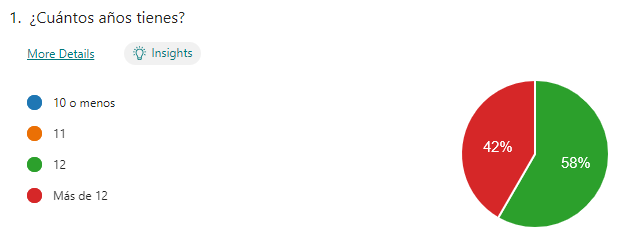
\includegraphics[width=450px,clip=true]{questionario_1.png}
  \caption{¿Cuántos años tienes?}
  \label{fig:questionario_1}
\end{figure}
\raggedbottom

\begin{figure}[H]
  \centering
  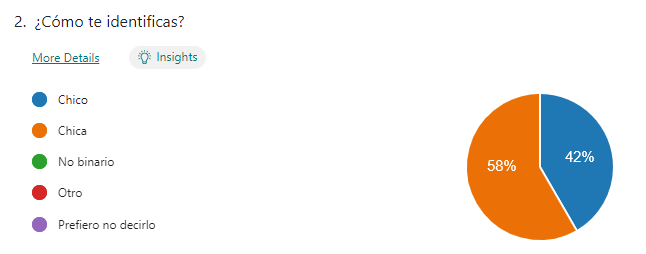
\includegraphics[width=450px,clip=true]{questionario_2.png}
  \caption{¿Cómo te identificas?}
  \label{fig:questionario_2}
\end{figure}
\raggedbottom

\begin{figure}[H]
  \centering
  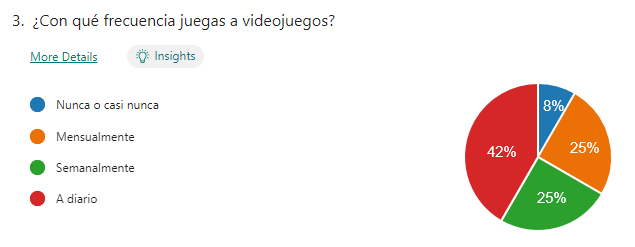
\includegraphics[width=450px,clip=true]{questionario_3.png}
  \caption{¿Con qué frecuencia juegas a videojuegos?}
  \label{fig:questionario_3}
\end{figure}
\raggedbottom

\begin{figure}[H]
  \centering
  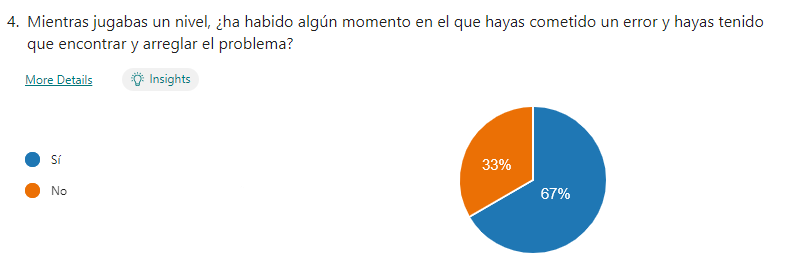
\includegraphics[width=450px,clip=true]{questionario_4.png}
  \caption{Mientras jugabas a un nivel, ¿ha habido algún momento en el que hayas cometido un error y hayas tenido que encontrar y arreglar el problema?}
  \label{fig:questionario_4}
\end{figure}
\raggedbottom

\begin{figure}[H]
  \centering
  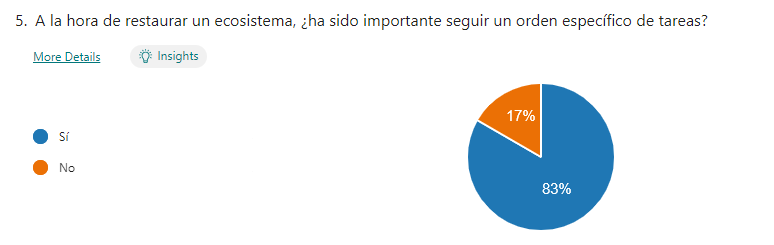
\includegraphics[width=450px,clip=true]{questionario_5.png}
  \caption{A la hora de restaurar un ecosistema, ¿Ha sido importante seguir un orden específico de tareas?}
  \label{fig:questionario_5}
\end{figure}
\raggedbottom

\begin{figure}[H]
  \centering
  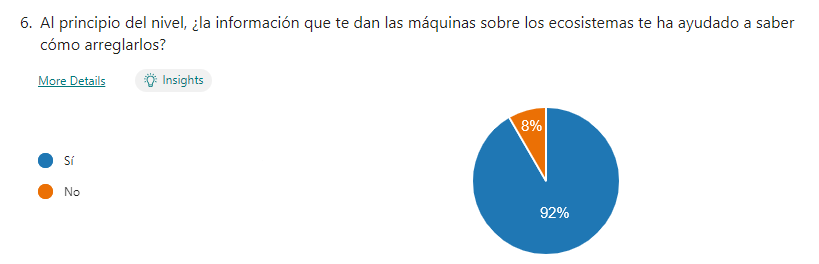
\includegraphics[width=450px,clip=true]{questionario_6.png}
  \caption{Al principio del nivel, ¿la información que te dan las máquinas sobre los ecosistemas te ha ayudado a saber cómo arreglarlos?}
  \label{fig:questionario_6}
\end{figure}
\raggedbottom

\begin{figure}[H]
  \centering
  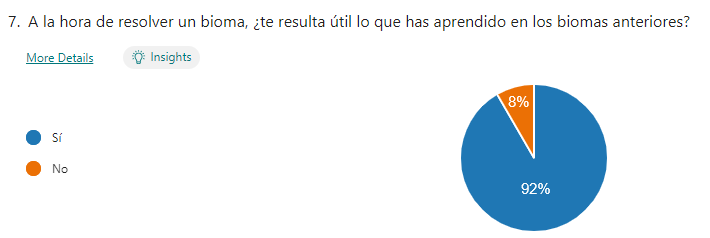
\includegraphics[width=450px,clip=true]{questionario_7.png}
  \caption{A la hora de resolver un problema, ¿te resulta útil lo que has aprendido en los biomas anteriores?}
  \label{fig:questionario_7}
\end{figure}
\raggedbottom

\begin{figure}[H]
  \centering
  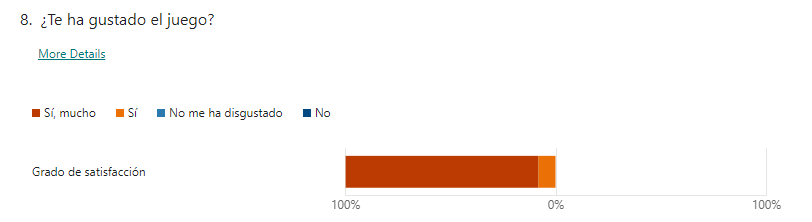
\includegraphics[width=450px,clip=true]{questionario_8.png}
  \caption{¿Te ha gustado el juego?}
  \label{fig:questionario_8}
\end{figure}
\raggedbottom

\begin{figure}[H]
  \centering
  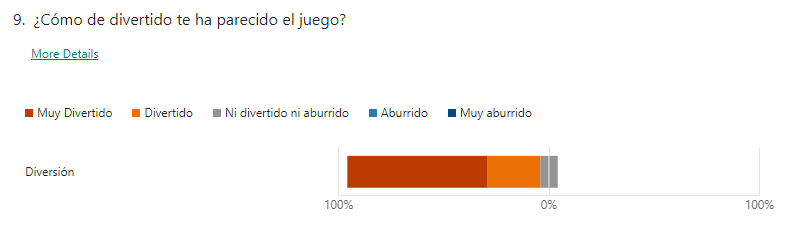
\includegraphics[width=450px,clip=true]{questionario_9.png}
  \caption{¿Cómo de divertido te ha parecido el juego?}
  \label{fig:questionario_9}
\end{figure}
\raggedbottom

\begin{figure}[H]
  \centering
  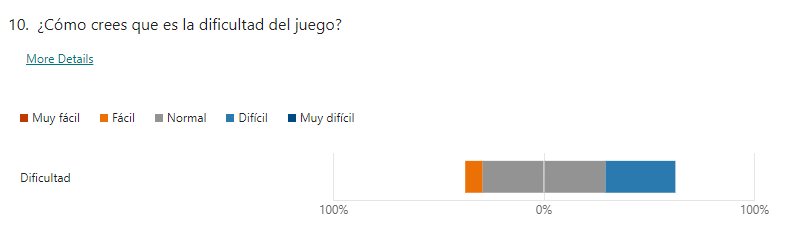
\includegraphics[width=450px,clip=true]{questionario_10.png}
  \caption{¿Cómo crees que es la dificultad del juego?}
  \label{fig:questionario_10}
\end{figure}
\raggedbottom

\begin{figure}[H]
  \centering
  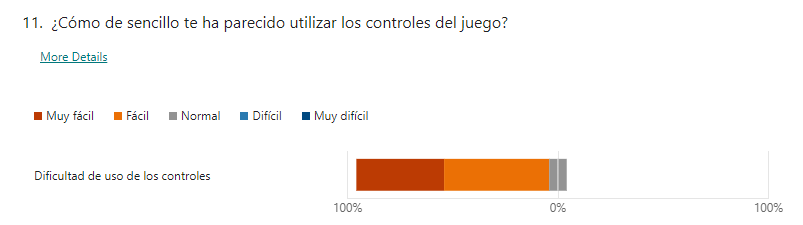
\includegraphics[width=450px,clip=true]{questionario_11.png}
  \caption{¿Cómo de sencillo te ha parecido utilizar los controles del juego?}
  \label{fig:questionario_11}
\end{figure}
\raggedbottom

\begin{figure}[H]
  \centering
  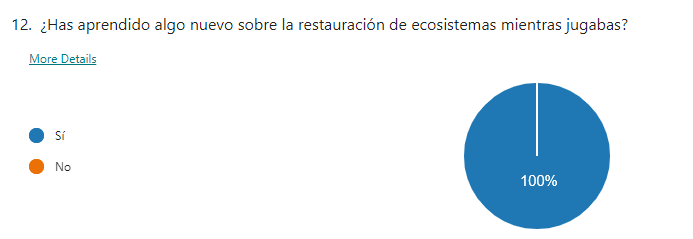
\includegraphics[width=450px,clip=true]{questionario_12.png}
  \caption{¿Has aprendido algo nuevo sobre la restauración de ecosistemas mientras jugabas?}
  \label{fig:questionario_12}
\end{figure}
\raggedbottom

\begin{table}[H]
  \begin{center}
  \setlength{\tabcolsep}{5pt}
  \renewcommand{\arraystretch}{1.2}
  \begin{tabular}{ | m{\textwidth} | } 
    \hline
    'La información que dan es muy útil' \\ 
    'He podido aprender mientras jugaba' \\ 
    'Me han gustado mucho los diseños, también me ha gustado cuando ponías las máquinas para ayudar al ecosistema' \\ 
    'La originalidad y poder aprender más sobre los ecosistemas' \\ 
    'Es fácil de usar y te explica muy bien las cosas' \\ 
    'Me ha gustado mucho la decoración y la base del juego, creo que es mucho más divertido comparado con los otros utensilios de clase' \\ 
    'Me gusta como iba subiendo la barra de progreso' \\ 
    'Las diferentes funciones de las máquinas' \\ 
    \hline
  \end{tabular}
  \centering
  \caption{¿Qué es lo que más te ha gustado del juego?}
  \label{fig:tablaResultadosPC}
  \end{center}
\end{table}  
 
\subsection{Datos Obtenidos por Telemetría}
\begin{table}[H]
  \begin{center}
  \setlength{\tabcolsep}{5pt}
  \renewcommand{\arraystretch}{1.2}
  \hspace*{-40px}
  \begin{tabular}{ @{} | m{2em} | m{4em} | m{3em} | m{2em} | m{4em} | m{4em} | m{4em} | m{3em} | m{3em} | m{4em} |  } 
  \hline
  ID & Name & Gender & Age & Progress & Machines Placed  & Machines Sold & Success Phase & Failure Phase & Duration \\
  \hline
  121  & 'Sandia' & 'Chica' &12 &0 &0 &0 &0 &0 &0  \\
  \hline
  121  & 'Sandia' & 'Chica' &12 &11 &2 &1 &1 &0 &2  \\
  \hline
  121  & 'Sandia' & 'Chica' &12 &22 &6 &4 &2 &3 &4  \\
  \hline
  121  & 'Sandia' & 'Chica' &12 &55 &9 &4 &5 &5 &6  \\
  \hline
  121  & 'Sandia' & 'Chica' &12 &100 &14 &5 &9 &9 &8  \\
  \hline
  122  & 'Ana' & 'Chica' &12 &0 &0 &0 &0 &0 &0  \\
  \hline
  122  & 'Ana' & 'Chica' &12 &22 &5 &3 &2 &2 &2  \\
  \hline
  122  & 'Ana' & 'Chica' &12 &44 &7 &3 &4 &4 &4  \\
  \hline
  122  & 'Ana' & 'Chica' &12 &100 &14 &5 &9 &9 &6  \\
  \hline
  123  & 'Ireee' & 'Chica' &13 &0 &0 &0 &0 &0 &0  \\
  \hline
  123  & 'Ireee' & 'Chica' &13 &33 &5 &2 &3 &2 &2  \\
  \hline
  123  & 'Ireee' & 'Chica' &13 &55 &8 &3 &5 &3 &4  \\
  \hline
  123  & 'Ireee' & 'Chica' &13 &100 &12 &3 &9 &5 &6  \\
  \hline
  124  & 'Bea' & 'Chica' &12 &0 &0 &0 &0 &0 &0  \\
  \hline
  124  & 'Bea' & 'Chica' &12 &33 &7 &4 &3 &2 &2  \\
  \hline
  124  & 'Bea' & 'Chica' &12 &44 &9 &5 &4 &3 &4  \\
  \hline
  124  & 'Bea' & 'Chica' &12 &100 &14 &5 &9 &5 &6  \\
  \hline
  125  & 'Leo' & 'Chico' &12 &0 &0 &0 &0 &0 &0  \\
  \hline
  125  & 'Leo' & 'Chico' &12 &22 &3 &1 &2 &0 &2  \\
  \hline
  125  & 'Leo' & 'Chico' &12 &33 &5 &2 &3 &3 &4  \\
  \hline
  125  & 'Leo' & 'Chico' &12 &55 &7 &2 &5 &4 &6  \\
  \hline
  126  & 'SALVA' & 'Chico' &13 &0 &0 &0 &0 &0 &0  \\
  \hline
  126  & 'SALVA' & 'Chico' &13 &33 &6 &3 &3 &2 &2  \\
  \hline
  126  & 'SALVA' & 'Chico' &13 &55 &8 &3 &5 &3 &4  \\
  \hline
  126  & 'SALVA' & 'Chico' &13 &100 &12 &3 &9 &5 &6  \\
  \hline
  127  & 'Calvo Pro' & 'Chico' &12 &0 &0 &0 &0 &0 &0 \\
  \hline
  127  & 'Calvo Pro' & 'Chico' &12 &22 &7 &5 &2 &1 &2 \\
  \hline 
  127  & 'Calvo Pro' & 'Chico' &12 &33 &8 &5 &3 &2 &4 \\
  \hline 
\end{tabular}
\centering
\end{center}
\end{table} 

\begin{table}[H]
  \begin{center}
  \setlength{\tabcolsep}{5pt}
  \renewcommand{\arraystretch}{1.2}
  \hspace*{-60px}
  \begin{tabular}{ @{} | m{2em} | m{4em} | m{3em} | m{2em} | m{4em} | m{4em} | m{4em} | m{3em} | m{3em} | m{4em} |  } 
  \hline
  128  & 'Virgy' & 'Chica' &12 &0 &0 &0 &0 &0 &0  \\
  \hline
  128  & 'Virgy' & 'Chica' &12 &33 &7 &4 &3 &2 &2  \\
  \hline
  128  & 'Virgy' & 'Chica' &12 &55 &9 &4 &5 &4 &4  \\
  \hline
  128  & 'Virgy' & 'Chica' &12 &100 &13 &4 &9 &5 &6  \\
  \hline
  129  & 'Sara' & 'Chica' &12 &0 &0 &0 &0 &0 &0  \\
  \hline
  129  & 'Sara' & 'Chica' &12 &33 &4 &1 &3 &2 &2  \\
  \hline
  129  & 'Sara' & 'Chica' &12 &44 &5 &1 &4 &3 &4  \\
  \hline
  129  & 'Sara' & 'Chica' &12 &100 &10 &1 &9 &7 &6  \\
  \hline
  130  & 'Paula' & 'Chica' &12 &0 &0 &0 &0 &0 &0  \\
  \hline
  130  & 'Paula' & 'Chica' &12 &11 &1 &0 &1 &1 &2  \\
  \hline
  130  & 'Paula' & 'Chica' &12 &33 &3 &0 &3 &2 &4  \\
  \hline
  130  & 'Paula' & 'Chica' &12 &77 &7 &0 &7 &6 &6  \\
  \hline
  131  & 'Pako' & 'Chico' &13 &0 &0 &0 &0 &0 &0  \\
  \hline
  132  & 'Pako' & 'Chico' &13 &22 &3 &1 &2 &1 &2  \\
  \hline
  133  & 'Pako' & 'Chico' &13 &55 &7 &2 &5 &2 &4  \\
  \hline
  134  & 'Pako' & 'Chico' &13 &66 &10 &4 &6 &5 &6  \\
  \hline
  135  & 'Pako' & 'Chico' &13 &66 &10 &4 &6 &6 &8  \\
  \hline
  136  & 'Pako' & 'Chico' &13 &66 &10 &4 &6 &7 &10  \\
  \hline
  137  & 'Pako' & 'Chico' &13 &66 &10 &4 &6 &8 &12  \\
  \hline
  138  & 'Pako' & 'Chico' &13 &66 &10 &4 &6 &9 &14  \\
  \hline
  139  & 'Pako' & 'Chico' &13 &66 &10 &4 &6 &11 &16  \\
  \hline
  140  & 'Pako' & 'Chico' &13 &66 &10 &4 &6 &12 &18  \\
  \hline
  141  & 'Pako' & 'Chico' &13 &66 &10 &4 &6 &12 &20  \\
  \hline
  147  & 'Paco' & 'Chico' &13 &0 &0 &0 &0 &0 &0  \\
  \hline
  147  & 'Paco' & 'Chico' &13 &11 &2 &1 &1 &0 &2  \\
  \hline
  147  & 'Paco' & 'Chico' &13 &33 &4 &1 &3 &1 &4  \\
  \hline
  147  & 'Paco' & 'Chico' &13 &66 &7 &1 &6 &5 &6  \\
  \hline
  147  & 'Paco' & 'Chico' &13 &100 &10 &1 &9 &8 &8  \\
  \hline
  148  & 'cali' & 'Chico' &13 &0 &0 &0 &0 &0 &0  \\
  \hline
  148  & 'cali' & 'Chico' &13 &22 &5 &3 &2 &2 &2  \\
  \hline
  148  & 'cali' & 'Chico' &13 &44 &7 &3 &4 &4 &4  \\
  \hline
  148  & 'cali' & 'Chico' &13 &100 &13 &4 &9 &5 &6  \\
  \hline
\end{tabular}
\centering
\end{center}
\end{table}  

\begin{table}[H]
  \begin{center}
  \hspace*{-40px}
  \begin{tabular}{ @{} | m{2em} | m{4em} | m{3em} | m{2em} | m{4em} | m{4em} | m{4em} | m{3em} | m{3em} | m{4em} |  } 
  \hline
  149  & 'Joselito' & 'Chico' &13 &0 &0 &0 &0 &0 &0  \\
  \hline
  150  & 'Joselito' & 'Chico' &13 &11 &2 &1 &1 &0 &2  \\
  \hline
  151  & 'Joselito' & 'Chico' &13 &22 &7 &5 &2 &0 &4  \\
  \hline
  152  & 'Joselito' & 'Chico' &13 &33 &8 &5 &3 &1 &6  \\
  \hline
  153  & 'Joselito' & 'Chico' &13 &55 &11 &6 &5 &1 &8  \\
  \hline
  154  & 'Joselito' & 'Chico' &13 &100 &15 &6 &9 &3 &10  \\
  \hline
\end{tabular}
\centering
\caption{Resultados obtenidos a partir de la Telemetría del Prototipo}
\label{fig:tablabbddpc}
\end{center}
\end{table}  


% También con \pagebreak

% Fin del documento
\end{document}
